% Novelty Audit Report — LaTeX edition
% Compile: pdflatex -> pdflatex (twice, for the table of contents)
\documentclass[11pt,a4paper]{article}

\usepackage[T1]{fontenc}
\usepackage[utf8]{inputenc}
\usepackage{lmodern}
\usepackage[margin=2.4cm]{geometry}
\usepackage{booktabs}
\usepackage{longtable}
\usepackage{array}
\usepackage{tabularx}
\usepackage{xcolor}
\usepackage{tcolorbox}
\usepackage{pgfplots}
\usepackage{enumitem}
\usepackage{microtype}
\usepackage{ragged2e}
\usepackage{titlesec}
\usepackage[htt]{hyphenat}   % allow hyphenation inside \texttt query strings
\usepackage[hidelinks]{hyperref}
\setlength{\emergencystretch}{3em}

\pgfplotsset{compat=1.17}
\tcbuselibrary{skins,breakable}

% ---------------------------------------------------------------- colours
\definecolor{ink}{HTML}{1B2430}
\definecolor{rule}{HTML}{C9D1D9}
\definecolor{killed}{HTML}{B3261E}
\definecolor{partial}{HTML}{C77700}
\definecolor{standing}{HTML}{1E6F5C}
\definecolor{clear}{HTML}{2B5CAB}
\definecolor{soft}{HTML}{F4F6F8}
\definecolor{softer}{HTML}{FAFBFC}

\color{ink}

% ---------------------------------------------------------------- headings
\titleformat{\section}{\Large\bfseries\color{ink}}{\thesection}{0.7em}{}
\titleformat{\subsection}{\large\bfseries\color{ink}}{\thesubsection}{0.6em}{}
\titlespacing*{\section}{0pt}{2.2ex plus 1ex minus .2ex}{1.2ex plus .2ex}

% ---------------------------------------------------------------- helpers
\newcommand{\vkilled}{\textcolor{killed}{\textbf{fully scooped}}}
\newcommand{\vpartial}{\textcolor{partial}{\textbf{partially scooped}}}
\newcommand{\vstanding}{\textcolor{standing}{\textbf{narrowed but standing}}}
\newcommand{\vclear}{\textcolor{clear}{\textbf{clear}}}
\newcommand{\readtag}{\textcolor{standing}{\textbf{[read in full]}}}
\newcommand{\abstag}{\textcolor{partial}{\textbf{[abstract only]}}}
\newcommand{\sniptag}{\textcolor{killed}{\textbf{[search result only]}}}
\newcommand{\unver}{\textcolor{killed}{\textsc{unverified}}}

\newtcolorbox{keybox}[1]{
  breakable, enhanced, colback=soft, colframe=ink, boxrule=0.4pt,
  left=10pt, right=10pt, top=8pt, bottom=8pt, arc=1pt,
  fonttitle=\bfseries, title={#1}}

\newtcolorbox{alertbox}[1]{
  breakable, enhanced, colback=softer, colframe=killed, boxrule=1.1pt,
  left=10pt, right=10pt, top=8pt, bottom=8pt, arc=1pt,
  fonttitle=\bfseries\color{white}, coltitle=white, colbacktitle=killed,
  title={#1}}

\newtcolorbox{quotebox}{
  breakable, enhanced, colback=soft, colframe=rule, boxrule=0pt,
  leftrule=3pt, colframe=ink,
  left=10pt, right=10pt, top=7pt, bottom=7pt, arc=0pt}

\setlist[itemize]{leftmargin=1.4em, itemsep=2pt, topsep=4pt}
\setlist[enumerate]{leftmargin=1.6em, itemsep=2pt, topsep=4pt}

\renewcommand{\arraystretch}{1.25}

% ================================================================
\begin{document}

\begin{titlepage}
\centering
\vspace*{2.5cm}
{\Huge\bfseries Novelty Audit\par}
\vspace{0.5cm}
{\LARGE Cross-Language Graph Federation\\[2mm] for Security Question Answering\par}
\vspace{1.4cm}
{\large An adversarial check of nine claims against the published literature\par}
\vspace{2.2cm}
\begin{minipage}{0.72\textwidth}
\centering
\rule{\textwidth}{0.4pt}\\[3mm]
{\large 26 August 2026}\\[3mm]
\rule{\textwidth}{0.4pt}
\end{minipage}
\vspace{2.2cm}

\begin{minipage}{0.78\textwidth}
\RaggedRight\small
Every claim in this report was treated as something to disprove rather than
support. Ninety-five distinct searches were run across three separate research
vocabularies. Forty-one documents were retrieved and read in full; fifteen more
were read only at the abstract, and are marked as such wherever they appear.
Nothing is cited here that was not opened, and every field that could not be
confirmed from a retrieved page is flagged.
\end{minipage}
\vfill
\end{titlepage}

\tableofcontents
\newpage

% ================================================================
\section{How to read this report}

Four labels are used throughout, and they mean different things.

\begin{center}
\begin{tabularx}{\textwidth}{@{}l>{\RaggedRight}X@{}}
\toprule
\vkilled & Someone has already published the claim. It cannot be presented as new. \\
\vpartial & Part of the claim is published. A narrower version survives, and this report says which. \\
\vstanding & The claim holds, but the wording has to change because some of its assumed territory is occupied. \\
\vclear & Nothing was found that occupies this ground. Note that this is a statement about what a search on a particular date found, not a proof of absence. \\
\bottomrule
\end{tabularx}
\end{center}

\vspace{4mm}

Sources carry one of three evidence labels:

\begin{itemize}
\item \readtag\ --- the whole document was retrieved and read. Claims about what a
      paper measured rest only on sources with this label.
\item \abstag\ --- only the summary page was retrieved. Such a source cannot be
      used as evidence about what a paper found.
\item \sniptag\ --- known only from a search listing. A lead to follow, not a finding.
\end{itemize}

Where a specific detail --- a journal name, a year, a list of authors, a number ---
could not be confirmed from a retrieved page, it is marked \unver.

% ================================================================
\section{Executive summary}

Three things break, and one of them is load-bearing.

\begin{alertbox}{1. The stated basis of the novelty claim does not exist}
The brief says that Sikos (2023), section 7, \emph{names} cross-source federation
for security and \emph{cites nothing for it}, and that this absence is ``the
current basis of our novelty claim.'' The paper was retrieved and read in full.
The word ``federat'' appears \textbf{exactly once in the entire article}, and the
worked example attached to it is not federation at all --- it is an ordinary
single-database query that reads from three named sections of one store. The
technical terms one would expect in a genuine discussion of federation
(\texttt{SERVICE}, ``endpoint'', ``interlink'') appear \textbf{zero times}. The
paper has no future-work or open-problems section anywhere.

Sikos is not flagging a gap. He is making a passing remark about a capability he
treats as already available. \textbf{This citation must be removed from the
novelty argument.} It does not support the sentence attached to it, and the
mismatch is discoverable in about ninety seconds by anyone who downloads the
paper --- which is precisely the failure this audit exists to prevent.
\end{alertbox}

\begin{alertbox}{2. Question 8 is dead}
A peer-reviewed journal article published on \textbf{28 July 2026 --- four weeks
before this audit} --- already covers the security of natural-language interfaces
to graph databases: an attack dataset, measures of unsafe and successful attacks,
enforcement that queries only read rather than write, and access control at the
boundary of the database's declared structure. This territory cannot be claimed.
\end{alertbox}

\begin{alertbox}{3. Question 3's method is taken, twice}
Mechanically identifying the earliest stage of a pipeline at which things went
wrong now exists in a peer-reviewed 2026 conference paper and in a 2026 preprint
that states the rule almost word for word. The \emph{finding} about where the
losses sit survives. The \emph{method} does not.
\end{alertbox}

Against that, four claims come through in usable shape, and two look genuinely
unoccupied.

\vspace{4mm}
\subsection*{Where the nine claims landed}

\begin{center}
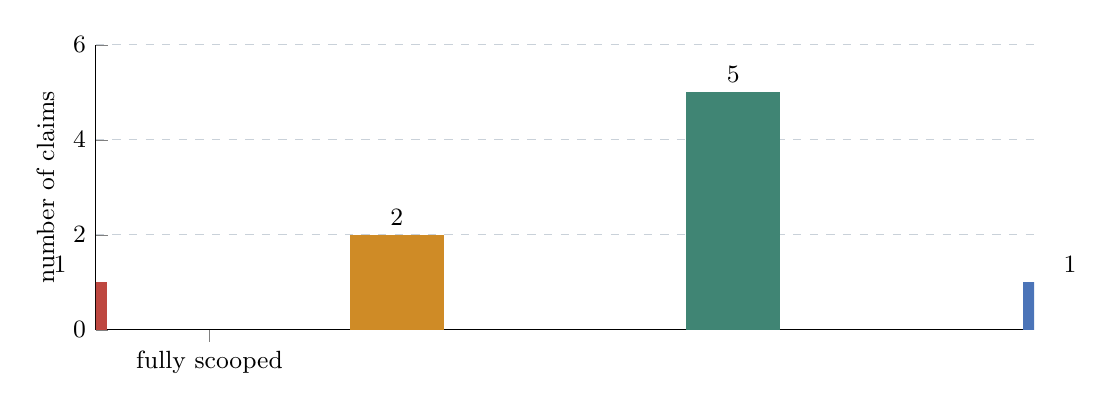
\begin{tikzpicture}
\begin{axis}[
  width=13.5cm, height=5.2cm,
  ybar, bar width=34pt,
  ymin=0, ymax=6,
  ylabel={number of claims},
  ylabel style={font=\small},
  symbolic x coords={{fully scooped},{partially scooped},{narrowed but standing},{clear}},
  xtick=data,
  xticklabel style={font=\small, align=center},
  yticklabel style={font=\small},
  ymajorgrids, grid style={rule, dashed},
  nodes near coords, nodes near coords style={font=\small\bfseries},
  axis lines*=left,
  enlarge x limits=0.16,
]
\addplot[fill=killed!85, draw=none] coordinates {({fully scooped},1)};
\addplot[fill=partial!85, draw=none] coordinates {({partially scooped},2)};
\addplot[fill=standing!85, draw=none] coordinates {({narrowed but standing},5)};
\addplot[fill=clear!85, draw=none] coordinates {({clear},1)};
\end{axis}
\end{tikzpicture}
\end{center}

\begin{keybox}{The one-line summary}
The architecture is not novel in kind --- a workshop paper from November 2025
already assembles most of it. What is novel is that nobody has \emph{measured}
any of this. The contribution is therefore the evaluation and the benchmark, not
the system design. That is a real contribution, but it is a different paper from
the one the brief appears to assume.
\end{keybox}

% ================================================================
\section{Verdict table}

\begin{center}
\footnotesize
\begin{longtable}{@{}p{0.6cm}>{\RaggedRight}p{2.7cm}>{\RaggedRight}p{2.2cm}>{\RaggedRight}p{4.1cm}>{\RaggedRight}p{2.9cm}>{\RaggedRight}p{1.2cm}@{}}
\toprule
\textbf{\#} & \textbf{Claim} & \textbf{Verdict} & \textbf{Closest published work} & \textbf{The difference} & \textbf{Conf.} \\
\midrule
\endfirsthead
\toprule
\textbf{\#} & \textbf{Claim} & \textbf{Verdict} & \textbf{Closest published work} & \textbf{The difference} & \textbf{Conf.} \\
\midrule
\endhead

Q1 & Answering questions by querying two graph stores that speak different query languages &
\vstanding &
Ozsoy, \emph{Toward Multi-Database Query Reasoning for Text2Cypher}, arXiv:2605.10373, 2026 --- \textbf{preprint} &
Proposes exactly this as a research roadmap and builds nothing; its evidence is seven hand-written questions, and its worked example pairs a graph language with a spreadsheet-style language, never two graph languages. & med.--high \\

Q2 & Comparing a federated against a merged system on \emph{answer accuracy} &
\vclear &
\emph{Samyama} biomedical graphs, arXiv:2603.15080, 2026 --- \textbf{preprint} \abstag &
Uses the word ``federation'' for what is actually merging everything into one store; one query language throughout; its accuracy table compares interfaces, not architectures. & medium \\

Q3 & Locating which pipeline stage lost the answer &
\vpartial &
Leung et al., \emph{Classifying and Addressing the Diversity of Errors in RAG Systems}, \textbf{EACL 2026} --- \textbf{peer-reviewed} &
They already walk the stages in order and stop at the first error --- but their pipeline has no planning stage, and their result runs the opposite way. & med.--high \\

Q4 & Hand-written query templates against structure-derived generic queries &
\vstanding &
Ding, Hu, Xu, Qu, \textbf{EMNLP-IJCNLP 2019} --- \textbf{peer-reviewed} &
Measures what templates cost in coverage, but never measures refusal and never leaves one database, so the reversal has no chance to appear. & medium \\

Q5 & Refusing to answer, and returning the query as proof &
\vpartial &
Sawhney et al., \textbf{Findings of ACL 2025} --- \textbf{peer-reviewed} &
Their task already outputs a valid query paired with ``no answer'', but scores it as a parse rather than offering it as something a reader is meant to check. & high \\

Q6 & Measuring how much a self-written test set inflates a score &
\vstanding &
Xu et al., \emph{When LLMs Benchmark Themselves}, arXiv:2509.26600, 2026 --- \textbf{preprint} &
They measure it when a \emph{language model} writes the questions; nobody measures it when a \emph{human research team} writes them for its own system. & high \\

Q7 & A query-level benchmark over the ATT\&CK or CAPEC catalogues &
\vstanding &
Simoni et al., \emph{TITAN}, arXiv:2510.14670, 2025 --- \textbf{preprint} &
Publishes 88{,}209 question--path pairs over an ATT\&CK graph, but its answers are chains of relationship names, not queries in any query language. & high \\

Q7b & No ATT\&CK/CAPEC question set with human-\emph{written} questions &
\vclear &
AttackQA (SambaNova) --- \textbf{preprint} &
Its ``human question'' column means a human wrote the \emph{generator script}. The trap flagged in the brief fired exactly as predicted. & high \\

Q8 & Security of natural-language interfaces to graph databases &
\vkilled &
Szlobodnyik, \emph{Analytics} 5(3):25, published \textbf{28 July 2026} --- \textbf{peer-reviewed journal} &
Already has the attack dataset, the safety measures, the read-only enforcement and the structure-boundary access control. Everything but a security-catalogue schema. & high \\

Q9 & Records from the wrong source reaching the answer &
\vstanding &
Arceo \& Narsing, \emph{Securing the Agent}, \textbf{ACM CAIS 2026} --- \textbf{peer-reviewed} &
They measure records the user was not \emph{allowed} to see; a record the user \emph{is} allowed to see but which came from the wrong source is never counted as a failure. & med.--high \\

\bottomrule
\end{longtable}
\end{center}

% ================================================================
\section{Corrections to the prior-art table}

Every row of the brief's section 2 was checked against a retrieved document. Four
of the eight rows are described inaccurately, and two of the inaccuracies matter.

\subsection{AgCyRAG --- closer than assumed, and two beliefs are wrong}

\readtag\ (CEUR-WS Vol-4079, paper 11, pp.~132--144).

\textbf{Corrected citation.} Kabul Kurniawan, Rayhan Firdaus Ardian, Elmar
Kiesling, Andreas Ekelhart. ``AgCyRAG: an Agentic Knowledge Graph based RAG
Framework for Automated Security Analysis.'' \emph{Second International Workshop
on Retrieval-Augmented Generation Enabled by Knowledge Graphs (RAGE-KG 2025)},
co-located with ISWC 2025, Nara, Japan, 2--6 November 2025. CEUR-WS Vol-4079,
pp.~132--144. Non-archival workshop paper; 21 submitted, 15 accepted.

There are \textbf{four} authors, and Ardian is \textbf{second}, not third. The
brief lists three names in the wrong order.

\paragraph{The belief about evaluation is right, and stronger than stated.}
There is no evaluation section, no measurements, no comparison systems, and no
numbers of any kind. Section 4.2 is titled ``Use Case Application'' and contains
three narrative walkthroughs, presented as coloured transcript boxes. The authors
say so themselves:

\begin{quotebox}
``For future work, we aim to conduct comprehensive evaluations of the framework
using a variety of LLM models (including local and specialized models), datasets,
and use cases\ldots''
\end{quotebox}

\paragraph{The belief about predefined queries is half wrong, and this matters.}
One of the two query languages is predefined; the other is written by a language
model on the fly.

\begin{quotebox}
``we implemented several predefined SPARQL queries in functions and exposed them
via MCP'' \hfill (section 4.1)

\vspace{3pt}
``the Cypher agent \textbf{generates} a Cypher query by means of an LLM to extract
structured, security-relevant relationships from the log graph.''
\end{quotebox}

Writing ``AgCyRAG uses predefined queries throughout'' will be caught by any
reviewer who opens the paper.

\paragraph{It is not federation in the technical sense.} Nothing is copied into a
common store, so that half of the description holds. But there is no query
decomposition and no join across the two stores. The two systems are consulted in
sequence by separate software agents, and their outputs are merged inside a prompt
to a language model. The defensible description is \emph{coordination across
separate stores by software agents}, not federation.

\begin{keybox}{Net effect}
The architectural sentence ``first system to issue queries in two graph languages
against separate, unmerged security stores'' is \textbf{already occupied}, by a
peer-reviewed workshop paper with public code. What is \emph{not} occupied is any
of it being measured.
\end{keybox}

\subsection{Sikos (2023) section 7 --- the belief is wrong, and this is the one that hurts}

\readtag\ (open access, full text).

\textbf{Corrected citation.} Leslie F. Sikos. ``Cybersecurity knowledge graphs.''
\emph{Knowledge and Information Systems} 65:3511--3531, 2023. Springer, open
access, \textbf{single author}, peer-reviewed journal survey.

Section 7 is titled ``Data aggregation and data fusion using cybersecurity
knowledge graphs.'' The entire textual basis for the claim is one sentence:

\begin{quotebox}
``By running federated queries on such a cyber-knowledge graph, entities having
certain property values according to data derived from multiple data sources
simultaneously can be found effectively.''
\end{quotebox}

Three problems, in ascending order of seriousness:

\begin{enumerate}
\item \textbf{The example attached to it is not federation.} It is a single query
      against a single store, reading from three internally named sections of that
      store. No remote system is contacted; nothing is distributed.
\item \textbf{The paragraph cites nothing} --- true, but because it is an offhand
      remark, not because a gap is being flagged.
\item \textbf{It describes an existing capability, not an open problem.} The paper
      has \emph{no} future-work or research-challenges section. Its conclusion is
      nine backward-looking sentences that cite nothing.
\end{enumerate}

\begin{alertbox}{What to do}
Delete this citation from the novelty argument. If a citation is wanted for
``cross-language security federation is unaddressed,'' it will have to be argued
from the \emph{pattern of absence} across the threat-intelligence systems
literature --- documented in the annotated bibliography of this report --- not from
a survey's non-existent gap statement.
\end{alertbox}

\subsection{FinAI Data Assistant --- retrieved, and its results are unusable}

\readtag\ (arXiv:2510.14162v2, full text).

\textbf{Corrected citation.} Juhyeong Kim, Yejin Kim, Youngbin Lee, Hyunwoo Byun.
``FinAI Data Assistant.'' arXiv:2510.14162. The document's own metadata declares
CIKM 2025. \textbf{The track is \unver} --- search evidence points to a CIKM 2025
\emph{workshop}, not the main conference. Do not cite it as a main-track paper.

\paragraph{The design idea is confirmed as prior art.} Section 3.2 describes
building a small set of parameterised base queries, wrapping each in a function
that validates its inputs, and letting a language model choose which function to
call and with what values. So ``route to vetted queries instead of writing them''
is in print ahead of you, in the spreadsheet-database modality.

\paragraph{But the deciding comparison has no numbers.} The section comparing this
approach against letting a model write queries contains \textbf{not a single
number in the text or in any table} --- everything lives inside a bitmap image. The
comparison system is never named, its failure rate is never quantified, and the
database is never specified. There is also no limitations section, despite the
summary promising one.

\begin{keybox}{Net effect}
They stake the idea; they do not defend it. Cite them for the design thesis, and
note in one sentence that their comparison is not quantitatively recoverable.
That is an accurate observation, not a cheap shot --- the numbers genuinely are not
in the paper.
\end{keybox}

\subsection{LinkQ --- a short paper with a demonstration, not an evaluation}

\readtag\ (arXiv:2406.06621 and the conference programme page).

\textbf{Corrected citation.} Harry Li, Gabriel Appleby, Ashley Suh. ``LinkQ.''
\textbf{IEEE VIS 2024 --- short paper track}, peer-reviewed.

\paragraph{The ``faithfulness guarantee'' is not a guarantee.} The mechanism is a
prompting loop: the system looks up the correct internal identifiers for the
entities in the question and places them in the model's instructions before it
writes a query. \textbf{Nothing checks that the query the model then writes
actually uses those identifiers.} That check is delegated to the human, via an
on-screen table ``intended to help users assess whether the LLM has identified the
correct IDs.'' The paper's own conclusion softens the summary's language to ``a
scalable protocol to \emph{reduce the frequency} of LLMs hallucinating.''

\paragraph{There is essentially no evaluation.} Section 5 is titled
``Demonstration'': five participants, six scripted questions. No standard
benchmark. No accuracy, precision, recall, or error rate. The entire quantitative
record is ``participants observed two inaccuracies'' and ``in 2/3 cases our system
successfully resulted in syntactically correct SPARQL queries and correct IDs.''
The authors write: ``In the future, we would like to quantitatively evaluate the
effectiveness of LinkQ\ldots''

\begin{keybox}{Net effect}
LinkQ is the closest prior art in \emph{intent}, and a far weaker artifact than its
reputation. A verifier that genuinely checks each claim against a retrieved record
is a stronger construct --- and, unlike LinkQ's, it can be measured.
\end{keybox}

\subsection{Graph-constrained reasoning --- ICML confirmed}

\readtag\ (proceedings page with citation record).

Linhao Luo, Zicheng Zhao, Gholamreza Haffari, \textbf{Yuan-Fang Li}, Chen Gong,
Shirui Pan. \emph{Proceedings of the 42nd International Conference on Machine
Learning (ICML 2025)}, vol.~267, pp.~41540--41565. The suspicion in the brief is
correct: \textbf{ICML, not ICLR}. Note that a widely circulated author list omits
Yuan-Fang Li. The results tables are \unver\ --- only the proceedings page and
summary were retrieved.

\subsection{The template family and constrained decoding --- all five confirmed}

All verified from retrieved bibliographic records. Bast \& Haussmann, CIKM 2015,
pp.~1431--1440. Zheng, Yu, Zou \& Cheng, PVLDB 11(11), 2018, pp.~1373--1386.
Abujabal, Yahya, Riedewald \& Weikum, WWW 2017, pp.~1191--1200. Gu, Pahuja, Cheng
\& Su, AKBC 2022 --- \textbf{no page numbers exist}; do not invent a range.
Scholak, Schucher \& Bahdanau (PICARD), EMNLP 2021 \textbf{main conference}, not
Findings, pp.~9895--9901.

% ================================================================
\newpage
\section{The nine claims, adjudicated}

\subsection{Q1. Two graph stores, two query languages --- \texorpdfstring{\vstanding}{narrowed but standing}}

Two sub-claims are dead; the core survives.

\paragraph{Dead: ``first to identify the problem.''} Makbule Gulcin Ozsoy (Neo4j),
arXiv:2605.10373, May 2026 --- \textbf{preprint}, \readtag. Its third phase is
verbatim ``heterogeneous query reasoning\ldots where multiple query languages\ldots
coexist.'' It also states ``to our knowledge, this problem remains largely
unexplored'' --- a sentence that is useful to cite and impossible to claim first.

But it builds nothing. It self-describes as ``a position paper proposing a research
roadmap rather than a fully implemented system,'' and its entire evidence base is
seven hand-written questions. Its multi-language example pairs a graph language
with a spreadsheet-style language, never two graph languages.

\paragraph{Dead: ``first natural-language-to-Gremlin.''} Yun et al.,
\emph{EICopilot}, arXiv:2501.13746, January 2025 --- \textbf{preprint}, \abstag. A
deployed system at a major search company that writes and runs Gremlin from plain
English, reporting 82.14\% execution correctness. One store, one language, one
domain --- but it forecloses any ``first'' framing on Gremlin.

\paragraph{Standing: the implemented, benchmarked, two-language, two-store system.}
Not found in a search of general web search, arXiv, CEUR-WS, the ACL Anthology and
Semantic Scholar on 26 August 2026, using 22 logged query strings across three
research vocabularies.

Two near-misses to pre-empt, because a reviewer will raise them:

\begin{itemize}
\item \textbf{UniQGen} (arXiv:2605.00845, 2026 --- preprint, \readtag) produces two
      different query languages from one pipeline and explicitly names the problem
      of being locked into one graph model. But both languages are sent to the
      \textbf{same} store. That is dual \emph{rendering}, not federation.
\item \textbf{Agentic SPARQL} (arXiv:2603.06582, 2026 --- preprint, \abstag) does
      genuine agent-driven federation over live endpoints. But its entire premise
      is that its one query language is standardised and federates natively, so the
      cross-language problem never arises. This is the strongest scoop risk in the
      semantic-web community for the \emph{agentic federated} half of the framing.
\end{itemize}

\begin{keybox}{Recommended wording}
``the first implemented and benchmarked system that answers natural-language
questions by dispatching native queries in two different graph query languages to
two live, unmerged graph stores.'' Cite Ozsoy, EICopilot, UniQGen and Agentic
SPARQL explicitly, or a reviewer will do it for you.
\end{keybox}

\textbf{Confidence: medium--high.} Residual risk sits in workshop proceedings,
which general web search indexes poorly, and arXiv's bulk search interface returned
empty results throughout, so no systematic sweep for the term ``Gremlin'' in
summaries was possible.

\subsection{Q2. Federated against merged, on answer accuracy --- \texorpdfstring{\vclear}{clear}}

Not found in a search of general web search, arXiv (summaries and full text),
CEUR-WS, the ACL Anthology, the ACM Digital Library, Springer, ScienceDirect and
PubMed Central on 26 August 2026, using eight targeted query strings, for any paper
that builds both a federated and a merged version of the \emph{same}
question-answering system and compares them on \textbf{answer accuracy}.

Two literatures were checked and both miss:

\begin{enumerate}
\item \textbf{Live-versus-copied data integration} in databases. Every comparison
      found is on \textbf{speed, cost, or how fresh the data is}. There is no
      correctness-of-answer axis anywhere in it.
\item \textbf{``Federated'' in the machine-learning sense.} Searches for
      federated-versus-centralised accuracy return \emph{federated learning} --- a
      completely different technique that happens to share the word. This deserves
      a defensive sentence, because a skimming reviewer will conflate them.
\end{enumerate}

\begin{keybox}{A terminology collision to pre-empt}
The Samyama preprint (arXiv:2603.15080, 2026, \abstag, authors \unver) calls itself
``cross-source federation'' while describing ``loading all three snapshots into a
single graph tenant'' --- that is, it uses ``federation'' to mean \emph{the merged
condition}. Its accuracy numbers compare \emph{interfaces}, not architectures.
\end{keybox}

\textbf{Confidence: medium.} This negative is genuinely hard to establish --- the
comparison could exist as an unlabelled table inside a paper whose title and
summary mention neither word. \textbf{Write ``we are not aware of,'' never ``no one
has compared these.''}

\subsection{Q3. Which stage lost the answer --- \texorpdfstring{\vpartial}{partially scooped}}

This is the claim that moved most during the audit, and it moved twice.

\paragraph{Scoop 1, peer-reviewed.} Leung, Belbahri, Sui, Labach, Zhang, Rose \&
Cresswell. \textbf{EACL 2026}, Long Papers, pp.~3185--3207. \readtag. (Venue
confirmed from a search listing rather than a retrieved page --- flagged.) From
their appendix:

\begin{quotebox}
``we proceed sequentially over the stages of the RAG pipeline in order, starting
with chunking. At each stage, an LLM is prompted with context to determine if an
error occurred at this stage\ldots \textbf{Once the earliest error is identified,
the evaluation stops.}''
\end{quotebox}

That is mechanical earliest-stage identification with a stopping rule. They then
report the resulting distribution over 832 and 1{,}222 failed responses, and
validate it by fixing the weak stages and re-running.

\textbf{Their result runs the opposite way,} which is the interesting part:

\begin{center}
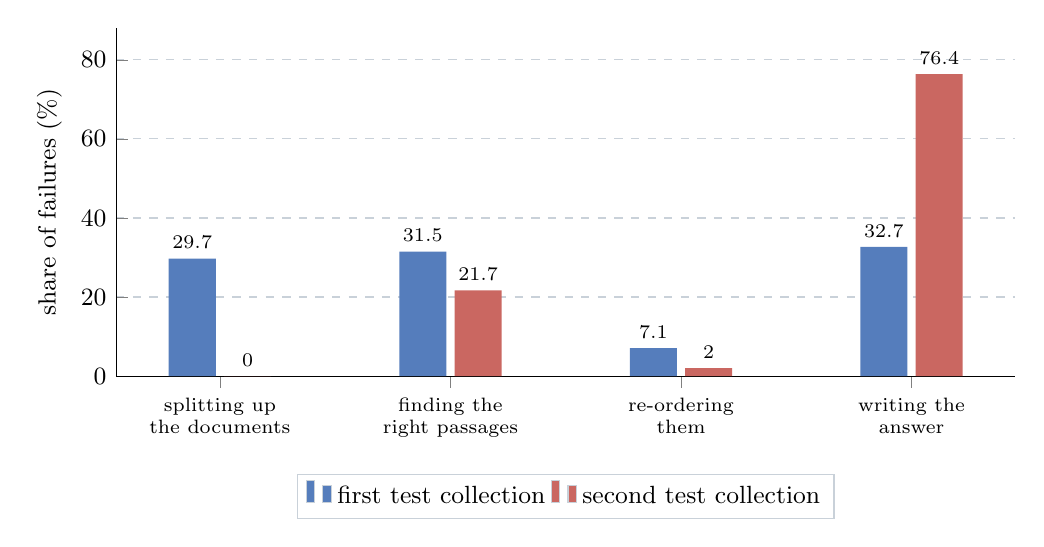
\begin{tikzpicture}
\begin{axis}[
  width=13cm, height=6cm,
  ybar=3pt, bar width=17pt,
  ymin=0, ymax=88,
  ylabel={share of failures (\%)},
  ylabel style={font=\small},
  symbolic x coords={{splitting up\\the documents},{finding the\\right passages},{re-ordering\\them},{writing the\\answer}},
  xtick=data,
  xticklabel style={font=\scriptsize, align=center},
  yticklabel style={font=\small},
  ymajorgrids, grid style={rule, dashed},
  legend style={font=\small, at={(0.5,-0.28)}, anchor=north, legend columns=2, draw=rule},
  nodes near coords, nodes near coords style={font=\scriptsize},
  axis lines*=left,
  enlarge x limits=0.15,
]
\addplot[fill=clear!80, draw=none] coordinates
  {({splitting up\\the documents},29.7) ({finding the\\right passages},31.5) ({re-ordering\\them},7.1) ({writing the\\answer},32.7)};
\addplot[fill=killed!70, draw=none] coordinates
  {({splitting up\\the documents},0) ({finding the\\right passages},21.7) ({re-ordering\\them},2.0) ({writing the\\answer},76.4)};
\legend{first test collection, second test collection}
\end{axis}
\end{tikzpicture}
\end{center}

The final stage --- writing the answer, which is where faithfulness failures live ---
is the largest single bucket in one setting and the overwhelming majority in the
other. The claim that faithfulness failures are a small minority is therefore not
merely unpublished; it \textbf{contradicts the only comparable published
distribution.} That is a strength if it can be explained (their pipeline has no
planning stage and no structured database; yours has both) and a liability if it
cannot.

\paragraph{Scoop 2: the localisation rule, stated almost verbatim.} Two 2026
preprints own it independently.

\emph{Causal Agent Replay}, arXiv:2606.08275 --- \textbf{preprint, single author},
\readtag:

\begin{quotebox}
``a \textbf{point-of-commitment rule: the causal locus is the latest step whose
effect's confidence interval still excludes zero---the last point at which
re-deciding still rescues the run}.''
\end{quotebox}

That is literally ``the last stage at which the correct answer was still
recoverable.'' But it is a debugging tool validated on artificial test cases with
planted answers; no knowledge graph, no query writing, and \textbf{no finding about
where losses concentrate in any real system}.

\emph{Doctor-RAG}, arXiv:2604.00865 --- \textbf{preprint, venue \unver}, \readtag\
(retrieved via the HTML view; the PDF has no machine-readable text). Its equation 3
defines the earliest erroneous action as a minimum over the trajectory, and treats
everything before it as a reusable valid prefix. Its error categories include a
\emph{search} type --- the closest published analogue to a planning stage. Its
distribution exists only inside an image, so those numbers are \unver.

One thin distinction survives: Doctor-RAG is \textbf{repair-oriented, not
recoverability-oriented} --- every located failure is assumed fixable by local
intervention, so it never asks whether the answer was still recoverable. That
distinction is too thin to build a contribution on.

\paragraph{One lead checked and cleared.} Ma et al., arXiv:2509.08682 (2025),
\readtag, does agent-level attribution and ``decisive error step'' prediction --- but
reports attribution \emph{accuracy} against labels, never a breakdown of what
fraction of failures originate where, and has no recoverability criterion.

\begin{alertbox}{A counter-example you must handle}
LogRouter (arXiv:2605.18015, 2026 --- preprint, authors \unver, \readtag) reports
routing accuracy alongside answer quality and states: ``\textbf{The relationship
between routing accuracy and answer quality is direct.}'' If you claim the routing
literature generally shows high routing accuracy alongside low answer accuracy,
this is the citation a reviewer will reach for. The Routing Plateau paper
(arXiv:2606.07587) fits the argument better, but note that its 10--30 point gap is
between a router and an ideal router --- a measure of selection quality, not a
routing-versus-answering discrepancy.
\end{alertbox}

\begin{alertbox}{Two statistics that must not be used}
Prose circulating in search results attributes ``planning\ldots representing 33\% of
total errors'' and ``29\% incorrect planning or decomposition / 47\% reasoning over
retrieved evidence / 10\% retrieval failures'' to a real paper. A dedicated tracing
pass could not resolve either to a retrievable document. The second was attributed
by a search engine to a journal article whose page returned an empty response, and
no preprint surfaced. \textbf{Not traced in a search of general web search, arXiv
and the ACM Digital Library on 26 August 2026}, using five logged query strings.
Treat both as probable search-engine synthesis. This is precisely the third
calibration error described in the brief.
\end{alertbox}

\textbf{Surviving claim:} mechanical last-recoverable-stage identification applied
to a \textbf{knowledge-graph} pipeline with an explicit \textbf{planning} stage,
yielding the finding that loss concentrates in planning while faithfulness failures
are a minority. Every component is published separately; the conjunction, and
specifically the \emph{direction} of the result, is not.

\subsection{Q4. Templates against generic construction --- \texorpdfstring{\vstanding}{narrowed but standing}}

\paragraph{The coverage half is already published.} Ding, Hu, Xu \& Qu,
\textbf{EMNLP-IJCNLP 2019}, peer-reviewed, \readtag\ including all result tables.
Their template comparison system scores 0.48 average accuracy against 0.846 for
their own method on the main test collection, and their diagnosis is explicit:
template systems' ``accuracy and coverage are limited by the rules and templates,''
and they ``cannot handle questions with unseen query structures, since they cannot
generate new query structures.''

\paragraph{Three things they do not do, and all three are yours.}

\begin{enumerate}
\item \textbf{They never measure refusal.} No split between answering and declining,
      no precision among answered questions. The concept does not appear.
\item \textbf{They never leave one database.} Both test collections sit on the same
      underlying structure, so there is no cross-structure condition in which a
      template precision advantage \emph{could} reverse.
\item \textbf{Their templates simply lose everywhere}, so the specific trade
      reported --- precision plus reliable refusal, paid for in coverage, with the
      precision edge inverting on an unfamiliar structure --- is not what they found.
\end{enumerate}

The reversal result was \textbf{not found in a search of general web search, the
ACL Anthology, arXiv, CEUR-WS and the EDBT open proceedings on 26 August 2026},
using seven exact query strings across three vocabularies; roughly nine to ten
results each, and zero returned a head-to-head measurement across structures.

\textbf{One adjacent paper that could be mistaken for a scoop:} SG-KBQA,
\textbf{EMNLP 2025}, peer-reviewed, \abstag\ --- \textbf{cannot be used as evidence
about its results.} From its summary, its comparisons are against other learned
systems rather than hand-written templates.

\textbf{Confidence: medium}, and the weakness is specific. The primary template
systems --- QUINT, TeBaQA, QAnswer/WDAqua --- were \textbf{not opened}. TeBaQA in
particular claims portability across databases, and a buried precision-versus-coverage
table there would narrow this further. \textbf{Open those four papers before
submitting.}

\subsection{Q5. Refusal that carries its proof --- \texorpdfstring{\vpartial}{partially scooped}}

\paragraph{The scoop.} Sawhney, Yadav, Bhattacharya \& Mausam,
\textbf{Findings of ACL 2025}, peer-reviewed, \readtag. Their task definition puts
the query in the refusal output: for questions the data cannot answer, the required
output is \textbf{a valid executable query paired with ``no answer.''} That is
exactly the artifact claimed.

\paragraph{Three deltas survive, and together they are a real contribution.}

\begin{enumerate}
\item \textbf{They score it; you show it.} The query is a parse evaluated by exact
      match. The paper contains no notion of a user; the word ``justification''
      never appears; there is no auditability or provenance discussion anywhere.
      Their own checking prompt treats an empty result as \emph{an error to repair}
      --- ``Please generate again a different executable sparql'' --- which is the
      precise opposite of treating it as evidence.
\item \textbf{Their structure-level refusal returns nothing.} When the question
      cannot be expressed against the database's structure at all, the system
      returns a bare label with zero evidentiary content. If your system returns an
      executed query even in that case, that case is unoccupied.
\item \textbf{The provenance connection is unmade.} A system combining database
      \emph{why-not} explanation --- the established technique for explaining why a
      record is missing from a result --- with a natural-language refusal decision was
      \textbf{not found in a search of general web search, arXiv, the ACL Anthology
      and database-conference indexes on 26 August 2026}, using 17 logged query
      strings. The two literatures remain disjoint. \textbf{That intersection is the
      strongest ground here.}
\end{enumerate}

\begin{keybox}{Reframe}
Frame the contribution as the \emph{evidentiary discipline}, not the output pair.
The pair is in Findings 2025.
\end{keybox}

\subsection{Q6. Self-written benchmark inflation --- \texorpdfstring{\vstanding}{narrowed but standing}}

\paragraph{The closest work measures the machine analogue, not yours.} Xu, Agrawal,
Zouhar, Freitag \& Deutsch, arXiv:2509.26600v2 --- \textbf{preprint only; no venue,
no acceptance statement}, \readtag. They separate self-favouring bias into a
test-set component and a grading component, isolating each with a clean design.

\begin{center}
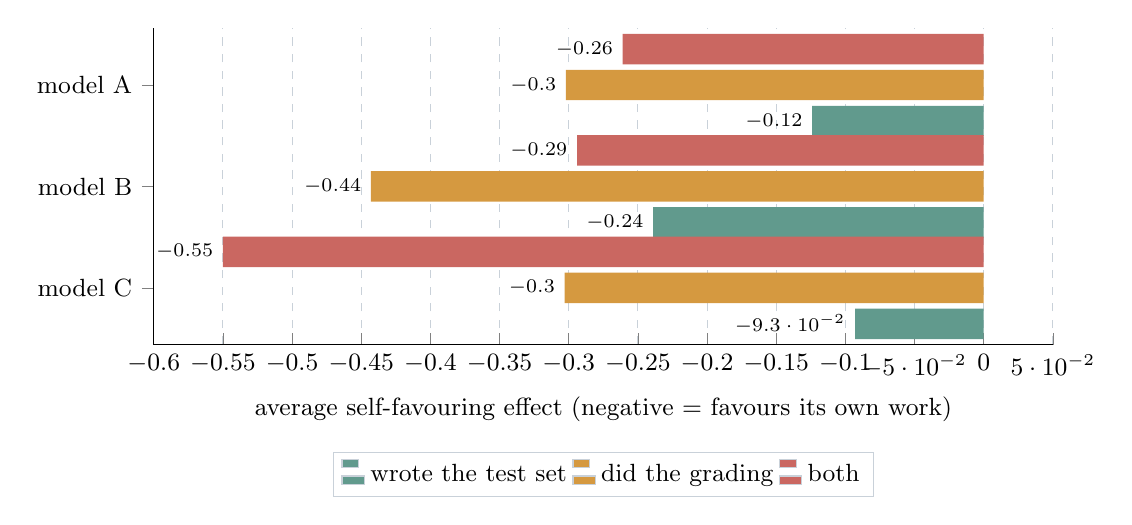
\begin{tikzpicture}
\begin{axis}[
  width=13cm, height=5.6cm,
  xbar=2pt, bar width=11pt,
  xmin=-0.6, xmax=0.05,
  xlabel={average self-favouring effect (negative = favours its own work)},
  xlabel style={font=\small},
  symbolic y coords={{model C},{model B},{model A}},
  ytick=data,
  yticklabel style={font=\small},
  xticklabel style={font=\small},
  xmajorgrids, grid style={rule, dashed},
  legend style={font=\small, at={(0.5,-0.34)}, anchor=north, legend columns=3, draw=rule},
  nodes near coords, nodes near coords style={font=\scriptsize},
  axis lines*=left,
  enlarge y limits=0.28,
]
\addplot[fill=standing!70, draw=none] coordinates {(-0.093,{model C}) (-0.239,{model B}) (-0.124,{model A})};
\addplot[fill=partial!75, draw=none] coordinates {(-0.303,{model C}) (-0.443,{model B}) (-0.302,{model A})};
\addplot[fill=killed!70, draw=none] coordinates {(-0.550,{model C}) (-0.294,{model B}) (-0.261,{model A})};
\legend{wrote the test set, did the grading, both}
\end{axis}
\end{tikzpicture}
\end{center}

Two caveats worth knowing. Their claim that the two components add together is
asserted but \textbf{not supported by their own table} --- for two of three systems
the combined figure is \emph{smaller} than the grading component alone. And they
never mention training-data contamination, so they neither test nor rule it out.

\paragraph{The delta is the author.} Their bias arises because a \emph{machine}
wrote the questions, and they attribute it to stylistic similarity. Yours arises
because a \emph{human research team} wrote them for its own system --- a different
agent, a different mechanism (design and framing choices rather than a stylistic
fingerprint), and a different unit (score points rather than rank positions). Their
paper treats human-written test sets only as a neutral control.

\paragraph{Three things this is not.} All are well covered; claim none of them.

\begin{center}
\begin{tabularx}{\textwidth}{@{}l>{\RaggedRight}X@{}}
\toprule
\textbf{Grader self-preference} & The grader favours text it wrote itself. Xu et al.\ measure it at two to three times the size of test-set bias. \\
\textbf{Training-data contamination} & The system saw the test questions during training. Retro-Holdouts reports up to 16 percentage points. \sniptag \\
\textbf{Selective disclosure} & Reporting only your best private run. \emph{The Leaderboard Illusion}, NeurIPS 2025, reports up to roughly 100 arena points. \sniptag \\
\bottomrule
\end{tabularx}
\end{center}

\paragraph{Two papers name the risk and measure nothing.} PeerBench
(arXiv:2510.07575, \abstag) warns that ``benchmark creators may collude with model
creators.'' \emph{Measuring what Matters} (NeurIPS 2025 Datasets \& Benchmarks,
\sniptag) reviews 445 benchmark papers and finds pervasive weaknesses in whether
benchmarks measure what they claim. Neither isolates developer authorship or
attaches a number. \textbf{PeerBench is the paper that would have scooped this and
did not.}

\begin{keybox}{Borrow the frame from medicine}
The mature, named, quantified version of this effect is \emph{industry sponsorship
bias} in clinical trials --- studies funded by a product's maker report more
favourable results than independent ones, and the size of that gap has been
measured repeatedly. Nobody appears to have ported it to machine-learning
benchmarking. Naming your effect against that precedent would strengthen the paper
considerably.
\end{keybox}

\subsection{Q7. A query-level security benchmark --- \texorpdfstring{\vstanding}{narrowed but standing}}

\paragraph{The belief as stated is too strong.} Three artifacts sit in the gap
claimed to be empty.

\textbf{The nearest.} Simoni, Fontanta, Saracino \& Mori, \emph{TITAN},
arXiv:2510.14670, 2025 --- \textbf{preprint, venue \unver}, \readtag. It releases
\textbf{88{,}209} question--path pairs over an ATT\&CK graph of 2{,}350 nodes and
48{,}795 edges. Never write ``no natural-language question resource exists over an
ATT\&CK graph.''

But its answers are chains of relationship names walked by a general-purpose Python
library. \textbf{No query language, no database, no execution-based scoring} --- only
exact string match plus text-similarity scores. No CAPEC. No human validation of any
generated example.

\textbf{Two others to cite.} CyKG-RAG (2024) and AgCyRAG (2025) \readtag\ both
generate queries over exactly these catalogues --- and ship \textbf{three anecdotal
example questions between them, zero reference queries, zero measurements.} And
CTIConnect (\textbf{KDD 2026}, peer-reviewed, \readtag) is the strongest
peer-reviewed baseline in this space --- 1{,}860 expert-\emph{verified} pairs across
five catalogues --- but retrieves by text similarity, with no query language and no
reference queries. Reviewers will expect engagement with it.

Meanwhile every real query-generation benchmark --- CypherBench, SpCQL,
MindTheQuery, SynthCypher, CyQuark --- has \textbf{zero security-catalogue content},
confirming that half of the belief.

\textbf{D3FEND and ATLAS:} no question set of any kind was located. Not found in a
search of general web search, arXiv, CEUR-WS, the ACL Anthology, the ACM Digital
Library and Hugging Face on 26 August 2026.

\begin{keybox}{Recommended wording}
``No benchmark exists that pairs natural-language questions with executable
reference queries in a standard graph query language, against a live graph store,
scored by whether executing them returns the right records, over MITRE ATT\&CK,
CAPEC, CVE, CWE, D3FEND or ATLAS.''
\end{keybox}

\subsection{Q7b. Human-written security questions --- \texorpdfstring{\vclear}{clear}, and the trap fired}

The calibration warning in the brief was exactly right, and it fired on the
most-cited candidate.

\begin{alertbox}{AttackQA's ``human question'' column does not mean what it says}
\readtag, section 3.3, verbatim:

\vspace{4pt}
``Twenty percent of the Q\&A pairs were generated by humans \textbf{using heuristics
embedded in code}, relying solely on the relationships table for their creation.''

\vspace{4pt}
That is a script iterating a table. A further 50\% are human-\emph{templated}
questions with machine-written answers; the remaining 30\% are fully machine-generated.
\textbf{Zero individually human-written questions.}
\end{alertbox}

Every other candidate falls the same way:

\begin{center}
\footnotesize
\begin{tabularx}{\textwidth}{@{}l>{\RaggedRight}X>{\RaggedRight}p{4.1cm}c@{}}
\toprule
\textbf{Dataset} & \textbf{Where the questions came from} & \textbf{What the humans did} & \textbf{Queries?} \\
\midrule
AttackQA \readtag & 20\% code templates, 50\% templated with machine answers, 30\% fully machine & scored a grader, not the questions & no \\
CTIBench \readtag & machine-generated from source pages; only \textbf{40 of 2{,}500} manually collected & checked and corrected a sample of $\sim$3{,}000 & no \\
CTIConnect \readtag & template-constrained machine synthesis from catalogue mappings & two practitioners plus an adjudicator \emph{verified} & no \\
TITAN \readtag & $\sim$700 hand-written templates, expanded and paraphrased & wrote templates; \textbf{no validation reported} & paths, not queries \\
Beyond RAG \readtag & machine-generated from machine-written queries over machine-extracted graphs & none --- conceded in limitations & never released or scored \\
SecBench \readtag & human contest entries plus automatic extraction from exams and books & experts assign quality tiers & no \\
ASU thesis \readtag & 30 genuinely author-written questions & author only & no --- prose similarity \\
\bottomrule
\end{tabularx}
\end{center}

\textbf{CTIBench's methodology is now verified rather than second-hand:} questions
were machine-generated from source pages, with roughly 3{,}000 sampled for manual
validation, unanswerable and multiply-correct items removed, and wrong annotations
corrected.

\textbf{SecBench is now closed too.} \readtag\ --- its 34{,}272 contest questions
\emph{are} genuinely human-written, and machines are confined to labelling and
grading. But its categories are nine self-devised domains, and \textbf{ATT\&CK,
CAPEC and CWE appear nowhere in the body, prompts or references.} There is no
ATT\&CK slice. It also skews heavily: 80.4\% of its questions are in Chinese, and
90.8\% test recall of facts.

\textbf{Verdict holds at clear.} The only genuinely hand-written ATT\&CK-adjacent
artifact found is a 30-question master's-thesis appendix with visible
question-to-answer misalignments.

\subsection{Q8. Security of natural-language graph interfaces --- \texorpdfstring{\vkilled}{fully scooped}}

\begin{alertbox}{Lead with this, because it collapses the claim}
Gergely Szlobodnyik. ``Feedback-Guided Prompt Injection Defense in
Retrieval-Augmented Text-to-Cypher Generation.'' \emph{Analytics} (MDPI), 2026,
5(3), 25. Peer-reviewed journal. Received 18 May 2026, accepted 21 July,
\textbf{published 28 July 2026 --- four weeks before this audit.} \readtag.
\end{alertbox}

It already contains, in one paper:

\begin{itemize}
\item a systematically constructed \textbf{attack dataset} across six categories of
      malicious instruction, built from sixteen parameterised templates;
\item an \textbf{unsafe-operation rate} and an \textbf{attack-success rate};
\item a \textbf{checking agent} that intercepts destructive queries and recovers ``a
      read-only, schema-consistent query'';
\item an identity-driven \textbf{access-control layer limiting execution to the
      authorised portion of the database's declared structure}, in both role-based
      and attribute-based forms;
\item a panel-of-models classifier labelling outputs faithful, malicious or diverged;
\item five foundation models and six comparison defences.
\end{itemize}

That is Q8, minus a security-catalogue schema.

\paragraph{What survives, and it is narrower than one would like.}

\begin{enumerate}
\item \textbf{Domain.} His evaluation uses a general-purpose corpus with a film
      database as the worked example. Nobody evaluates over a \textbf{security
      catalogue}, where the data itself describes attacks and the structural boundary
      \emph{is} a classification boundary.
\item \textbf{Language.} No adversarial probe suite exists for \textbf{Gremlin}.
\item \textbf{Level of enforcement.} His defence operates at the prompt and checker
      level; it is never tested against \textbf{database-level permissions} or
      execution on a live store.
\item \textbf{Who wrote the probes.} His attack templates are machine-authored, so an
      \textbf{analyst-authored} probe suite is unclaimed --- and note this dovetails
      neatly with the Q6 argument about who writes the test set.
\end{enumerate}

\paragraph{Second required citation.} Hamzić, Skopik, Landauer, Wurzenberger \&
Rauber, arXiv:2604.11419, April 2026 --- \textbf{preprint}, \readtag. Contributes
read-only restriction as a \emph{prompt} constraint, a \textbf{structure-evasion
attack with an 82.5\% success rate}, a ``structural hallucination'' failure mode,
a refusal/overconfidence table, and a \textbf{timing side channel} (failed queries
292.6 seconds against 45.0 successful, a 6.5-fold ratio). Note its ``3{,}300
question-answer pairs'' is 660 unique questions run through 5 systems.

Also worth one line each: \textbf{CVE-2024-7042}, a real query-injection
vulnerability in a widely used open-source toolkit (\sniptag), as evidence the
problem class occurs in deployed software; and vendor production guidance on
read-only accounts, timeouts and automatic result limits (\sniptag), which
establishes that these mitigations currently circulate as folklore rather than
measurement --- an argument \emph{for} a measurement paper.

\subsection{Q9. Records from the wrong source --- \texorpdfstring{\vstanding}{narrowed but standing}}

The \textbf{permission} axis is now peer-reviewed and well covered. The
\textbf{provenance} axis described in the brief is not.

\paragraph{The closest work.} Arceo \& Narsing (Red Hat AI), \textbf{ACM Conference
on AI and Agentic Systems 2026}, peer-reviewed, \readtag. They formalise the gap
between what is \emph{relevant} and what a user is \emph{allowed to see}, and
measure leakage across tenants: 98--100\% of probes leak without gating, 0\% with
gating; 62--80\% leakage on 90 attack probes ungated.

\textbf{But their failure test is strictly ``was the user allowed to see this?''}
--- within a \textbf{single shared index} over a synthetic 300-document corpus. A
record the user \emph{is} allowed to see, which came from the wrong source, counts
at worst as a precision loss and never as a violation. No fan-out across stores, no
graph retrieval, no released probe suite.

\paragraph{Two adjacent papers ruled out by direct reading.}

\begin{itemize}
\item Mu \& Li, arXiv:2605.28112, 2026 --- preprint, \readtag. Has the exact fan-out
      architecture, but the wrong source is wrong because it is \textbf{malicious},
      not honest-but-off-topic. No leakage measure at all.
\item Burnat \& Davidson, arXiv:2605.19847, 2026 --- preprint, \readtag. Explicitly
      forbids the multi-store case: ``each query is scored against only that
      account's tenant index,'' and cross-tenant leakage is ``zero by design.'' Its
      ``each action legal, aggregate illegal'' structure is the right \emph{shape} on
      the wrong \emph{axis} --- accounts, not sources.
\end{itemize}

\begin{keybox}{The gap in this negative is now closed}
FeB4RAG --- Wang, Khramtsova, Zhuang \& Zuccon, \textbf{SIGIR 2024}, pp.~763--773
(metadata \unver\ by fetch; full text \readtag) --- was the single most plausible
hiding place for a cross-source measure. It is not there. A full-text search for
\emph{contaminat}, \emph{confidential}, \emph{privacy}, \emph{leakage},
\emph{cross-source}, \emph{provenance} and \emph{attribution} returns
\textbf{zero matches}. Its measures are standard ranking-quality scores over 790
requests and 16 engines.
\end{keybox}

\textbf{Surviving claim:} no published work defines or measures a
\textbf{cross-source contamination rate} for the case where one question fans out
to several distinct stores, each sub-query is individually authorised for the store
it hits, and the aggregate answer mixes provenance. The nearest measures are all
one-sided.

% ================================================================
\newpage
\section{Scoop watch, ranked by threat}

\begin{center}
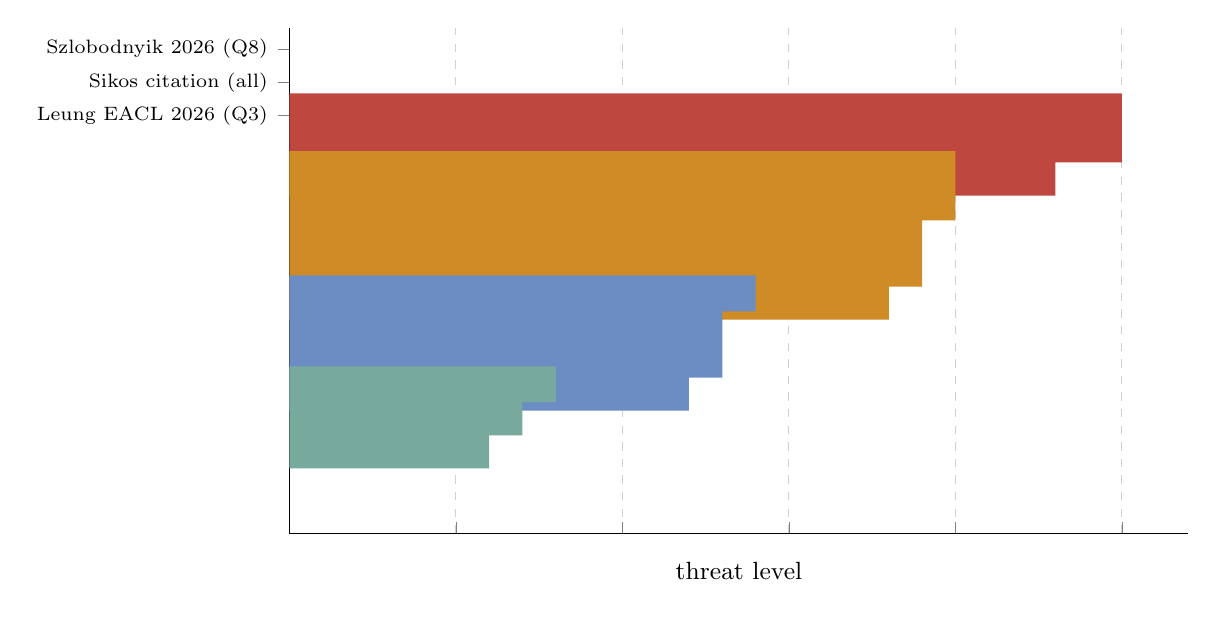
\begin{tikzpicture}
\begin{axis}[
  width=13cm, height=8cm,
  xbar, bar width=13pt,
  xmin=0, xmax=5.4,
  xlabel={threat level},
  xlabel style={font=\small},
  symbolic y coords={
    {Ding 2019 (Q4)},
    {LogRouter (Q3)},
    {UniQGen / EICopilot (Q1)},
    {TITAN (Q7)},
    {Sawhney 2025 (Q5)},
    {CTIConnect KDD 2026 (Q7)},
    {Xu 2026 (Q6)},
    {Shah CAR (Q3)},
    {Arceo \& Narsing (Q9)},
    {Ozsoy 2026 (Q1)},
    {AgCyRAG (Q1/Q7)},
    {Doctor-RAG (Q3)},
    {Leung EACL 2026 (Q3)},
    {Sikos citation (all)},
    {Szlobodnyik 2026 (Q8)}},
  ytick=data,
  yticklabel style={font=\scriptsize},
  xtick={1,2,3,4,5},
  xticklabels={,,,,},
  xmajorgrids, grid style={rule, dashed},
  axis lines*=left,
  enlarge y limits=0.045,
]
\addplot[fill=killed!85, draw=none] coordinates {(5,{Szlobodnyik 2026 (Q8)}) (5,{Sikos citation (all)}) (4.6,{Leung EACL 2026 (Q3)})};
\addplot[fill=partial!85, draw=none] coordinates {
  (4.0,{Doctor-RAG (Q3)}) (4.0,{AgCyRAG (Q1/Q7)}) (3.8,{Ozsoy 2026 (Q1)})
  (3.8,{Arceo \& Narsing (Q9)}) (3.6,{Shah CAR (Q3)})};
\addplot[fill=clear!70, draw=none] coordinates {
  (2.8,{Xu 2026 (Q6)}) (2.6,{CTIConnect KDD 2026 (Q7)}) (2.6,{Sawhney 2025 (Q5)})
  (2.4,{TITAN (Q7)})};
\addplot[fill=standing!60, draw=none] coordinates {
  (1.6,{UniQGen / EICopilot (Q1)}) (1.4,{LogRouter (Q3)}) (1.2,{Ding 2019 (Q4)})};
\end{axis}
\end{tikzpicture}
\end{center}

\begin{center}
\footnotesize
\begin{longtable}{@{}c>{\RaggedRight}p{5.6cm}c>{\RaggedRight}p{6.4cm}@{}}
\toprule
\textbf{\#} & \textbf{Work} & \textbf{Hits} & \textbf{What to do} \\
\midrule
\endfirsthead
\toprule
\textbf{\#} & \textbf{Work} & \textbf{Hits} & \textbf{What to do} \\
\midrule
\endhead
1 & Szlobodnyik, \emph{Analytics} 5(3):25, published 28 July 2026 --- peer-reviewed journal \readtag & Q8 & The generic framing is dead. Rewrite as catalogue-specific, or cut to a paragraph. Must cite. \\
2 & \textbf{Sikos 2023 does not say what the brief thinks} \readtag & all & Remove the citation. Rebuild the gap argument from the pattern of absence. \\
3 & Leung et al., EACL 2026 --- peer-reviewed \readtag & Q3 & Method scooped, and their distribution contradicts yours. Cite, and explain the difference structurally. \\
4 & Doctor-RAG, arXiv:2604.00865 --- preprint \readtag & Q3 & Earliest-error location with a \emph{search} error category --- the closest published analogue to a planning stage. \\
5 & AgCyRAG, workshop at ISWC 2025 \readtag & Q1, Q7 & Occupies the architecture. Correct the description of it before a reviewer does. \\
6 & Ozsoy, arXiv:2605.10373 --- preprint \readtag & Q1 & Owns the problem statement. Cite and position against; you own the implementation. \\
7 & Arceo \& Narsing, ACM CAIS 2026 --- peer-reviewed \readtag & Q9 & Owns the permission axis with hard numbers. Position yours as the orthogonal provenance axis. \\
8 & Shah, \emph{Causal Agent Replay} --- preprint \readtag & Q3 & States the localisation rule almost verbatim. Must cite. \\
9 & Simoni et al., \emph{TITAN} --- preprint \readtag & Q7 & Never say ``no ATT\&CK question resource exists.'' Scope to query language and execution scoring. \\
10 & Sawhney et al., Findings of ACL 2025 --- peer-reviewed \readtag & Q5 & Owns the output pair. Reframe around evidentiary discipline and the structure-level case. \\
11 & Xu et al., arXiv:2509.26600 --- preprint \readtag & Q6 & Measures the machine-authored analogue. Cite, then distinguish the human mechanism. \\
12 & Cheng et al., CTIConnect, KDD 2026 --- peer-reviewed \readtag & Q7, Q9 & Strongest peer-reviewed baseline, with a live leaderboard. Engage or be asked why not. \\
13 & Hamzić et al., arXiv:2604.11419 --- preprint \readtag & Q7, Q8 & Structure-evasion taxonomy, refusal table, timing side channel. Watch for a venue. \\
14 & Dobriy et al., \emph{Agentic SPARQL} --- preprint \abstag & Q1 & Owns agent-driven federation in the semantic-web community. Cross-language is what distinguishes you. \\
15 & \textbf{The Kurniawan/Kiesling/Ekelhart group itself} \readtag & Q1, Q7, Q8 & They have said in \emph{two consecutive papers} that evaluation is future work. That is your benchmark, unbuilt, by an active group. \\
16 & Ding et al., EMNLP-IJCNLP 2019 \readtag & Q4 & Owns the coverage half. Cite as the baseline your results extend. \\
17 & UniQGen; EICopilot \readtag / \abstag & Q1 & Foreclose two ``first'' claims. Cite both. \\
18 & LogRouter --- preprint \readtag & Q3 & A published counter-example to the routing sub-claim. Soften that sentence. \\
19 & Leaderboard Illusion; Measuring what Matters; PeerBench \sniptag / \abstag & Q6 & Adjacent framings a reviewer will name. Distinguish each in one sentence. \\
20 & CyQuark, CypherBench, SpCQL, MindTheQuery and others \readtag / \sniptag & Q7 & Zero security content today, but a domain-transfer paper is cheap for them to write. \\
\bottomrule
\end{longtable}
\end{center}

% ================================================================
\newpage
\section{The surviving claim, and the attack on it}

\subsection{The strongest honest statement}

\begin{keybox}{What can be claimed}
We present the first implemented and empirically evaluated system that answers
natural-language questions by dispatching native queries in two different graph
query languages to live, independently administered stores that are never merged,
joined at answer time through a declared key with identifier reconciliation across
two identifier schemes. Because the system writes no queries with a language model,
we can measure things that generation-based architectures cannot isolate: we
identify the last pipeline stage at which the correct answer remained recoverable
and find that loss concentrates in planning rather than in query construction or
answer writing; we compare hand-written templates against structure-derived generic
queries across two databases and find that the precision advantage of templates
reverses on a database for which no templates were written; we compare a federated
against a merged configuration of the same system and find no accuracy advantage
for either; and we quantify the score inflation contributed by a question set
written alongside the system that answers it. We contribute the first question set
over the ATT\&CK and CAPEC catalogues that pairs natural-language questions with
executable reference queries scored by execution.
\end{keybox}

Note what has been removed: any claim to have identified the cross-language problem
first, any claim to first Gremlin generation, any claim about the security of
natural-language graph interfaces, and any appeal to Sikos as evidence of a gap.

\subsection{The sentence a hostile reviewer will use}

\begin{alertbox}{The attack}
``The architecture is AgCyRAG with a different second query language and a benchmark
attached; the cross-language framing was proposed by Ozsoy in 2026; and the
individual mechanisms --- templates instead of parsing, earliest-stage error
attribution, refusal returning a query, read-only enforcement on generated graph
queries --- are each published elsewhere. The contribution is an engineering
integration whose headline empirical results are three null findings.''
\end{alertbox}

\subsection{Can it be answered?}

\textbf{Partly --- and the honest answer is that it depends entirely on the
evaluation, not on the architecture.}

\paragraph{What can be said.} AgCyRAG writes its second query language with a
language model, reports no numbers of any kind, and is not a federation in the
technical sense. Ozsoy explicitly builds nothing and never pairs two graph
languages. And a system that eliminates query generation is a \emph{different
measuring instrument}, not merely a different implementation --- it is what makes
stage-wise attribution and the template comparison possible at all, because there
is no random query-writing step to confound them.

\paragraph{What cannot be said.} That the architecture is novel in kind. It is not.
Nor can the failure-attribution \emph{method} be claimed.

\begin{alertbox}{The strategic implication}
The architecture is the method section, not the contribution. The contribution is
four measurements --- three of which are nulls --- plus the benchmark. Papers built
on null results need unusually clean design and unusually careful claims, and one
of the nulls currently \textbf{contradicts} the only comparable published
distribution. Explaining that contradiction structurally, rather than waving at it,
is the single highest-value thing to do before submission.

\vspace{4pt}
\textbf{One reframing worth considering:} the benchmark may be the stronger paper. It
is the cleanest gap this audit found, and it is exactly what the most active
competing group has twice declared to be future work.
\end{alertbox}

% ================================================================
\newpage
\section{What to stop claiming}

\begin{center}
\footnotesize
\begin{longtable}{@{}>{\RaggedRight}p{4.8cm}>{\RaggedRight}p{5.4cm}>{\RaggedRight}p{5.2cm}@{}}
\toprule
\textbf{Stop claiming} & \textbf{Because} & \textbf{Replace with} \\
\midrule
\endfirsthead
\toprule
\textbf{Stop claiming} & \textbf{Because} & \textbf{Replace with} \\
\midrule
\endhead
That Sikos (2023) names cross-source federation for security as an uncited gap & The word appears once, uncited, describing an ordinary single-store query as an existing capability; there is no future-work section & Argue the gap from the pattern of absence across the threat-intelligence systems literature; cite Ozsoy (2026) for the explicit problem statement \\
That the security of natural-language graph interfaces is unaddressed & Szlobodnyik, published 28 July 2026, peer-reviewed, covers all four mechanisms & Narrow to security catalogues, Gremlin, database-level enforcement, or analyst-written probes --- or cut to a paragraph \\
That AgCyRAG uses predefined queries throughout & Its second query language is machine-generated; only the first is predefined & ``AgCyRAG predefines its access to one store and generates its queries to the other'' \\
That AgCyRAG is a federated system & No decomposition, no cross-store join; integration happens in the prompt & ``coordination across separate stores by software agents'' \\
Priority on identifying cross-language federation & Ozsoy, May 2026 & Priority on \emph{implementing and measuring} it \\
First natural-language-to-Gremlin & EICopilot, January 2025, deployed & First to route to Gremlin \emph{as one of two languages in a federated plan} \\
That no question resource exists over an ATT\&CK graph & TITAN, 88{,}209 pairs, 2025 & No resource pairs questions with executable reference queries scored by execution \\
That returning the query on refusal is unprecedented & Findings of ACL 2025 defines exactly that output & The query as a \emph{reader-checkable} artifact, plus the structure-level case, plus the why-not connection \\
That mechanical stage-wise failure location is new & EACL 2026 and Doctor-RAG both do it & The \emph{finding} --- planning-dominant loss --- not the mechanism \\
That routing work generally shows high routing accuracy with low answer accuracy & LogRouter reports the relationship is direct & Cite the Routing Plateau's ideal-router gap instead, with the caveat stated \\
That LinkQ offers a faithfulness \emph{guarantee} & Nothing checks the emitted query against the supplied identifiers & ``a design goal of reducing hallucination frequency, evaluated qualitatively'' \\
\bottomrule
\end{longtable}
\end{center}

% ================================================================
\newpage
\section{Search log}

All searches were run on \textbf{26 August 2026} through a general web search tool,
with primary sources retrieved by direct fetch. ``Rel.''\ counts results judged
worth opening.

\begin{center}
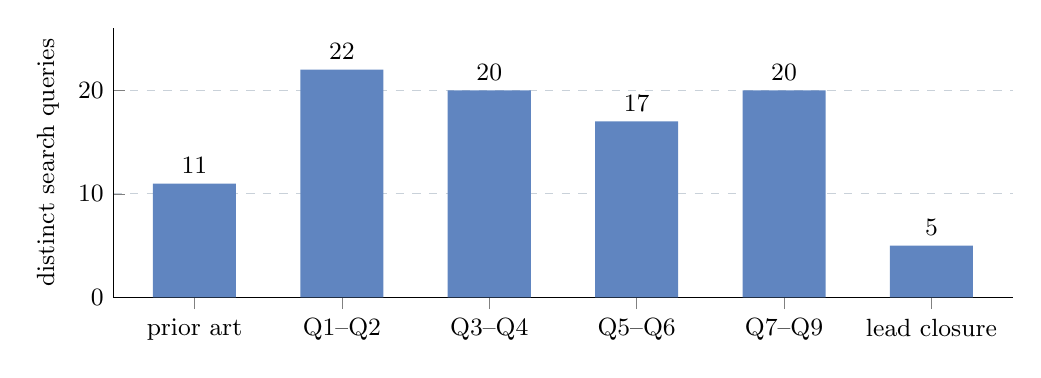
\begin{tikzpicture}
\begin{axis}[
  width=13cm, height=5cm,
  ybar, bar width=30pt,
  ymin=0, ymax=26,
  ylabel={distinct search queries},
  ylabel style={font=\small},
  symbolic x coords={{prior art},{Q1--Q2},{Q3--Q4},{Q5--Q6},{Q7--Q9},{lead closure}},
  xtick=data,
  xticklabel style={font=\small},
  yticklabel style={font=\small},
  ymajorgrids, grid style={rule, dashed},
  nodes near coords, nodes near coords style={font=\small\bfseries},
  axis lines*=left,
  enlarge x limits=0.11,
]
\addplot[fill=clear!75, draw=none] coordinates
  {({prior art},11) ({Q1--Q2},22) ({Q3--Q4},20) ({Q5--Q6},17) ({Q7--Q9},20) ({lead closure},5)};
\end{axis}
\end{tikzpicture}
\end{center}

\begin{center}
\textbf{Total: 95 distinct queries across three research vocabularies.}
\end{center}

\subsection{Prior-art verification (11 queries)}

\begin{center}
\footnotesize
\begin{tabularx}{\textwidth}{@{}c>{\RaggedRight}Xc@{}}
\toprule
\textbf{\#} & \textbf{Query string} & \textbf{Rel.} \\
\midrule
1 & \texttt{AgCyRAG Kurniawan Kiesling Ekelhart agentic RAG cybersecurity knowledge graph} & 3 \\
2 & \texttt{RAGE-KG workshop ISWC 2025 CEUR proceedings retrieval augmented generation knowledge graphs} & 5 \\
3 & \texttt{"FinAI Data Assistant" LLM parameterized SQL queries routing paper} & 3 \\
4 & \texttt{LinkQ LLM knowledge graph question answering SPARQL faithfulness arXiv} & 3 \\
5 & \texttt{graph-constrained reasoning KG-Trie Luo faithful LLM reasoning knowledge graph ICML 2025} & 6 \\
6 & \texttt{"FinAI Data Assistant" CIKM 2025 ACM proceedings Kim Byun} & 4 \\
7 & \texttt{LinkQ "IEEE" visualization 2024 knowledge graph question answering VIS} & 4 \\
8 & \texttt{Sikos "Cybersecurity knowledge graphs" 2023 Knowledge and Information Systems survey federation SPARQL} & 5 \\
9 & \texttt{2026 agentic LLM cybersecurity knowledge graph question answering multiple graph stores Cypher SPARQL federation} & 4 \\
10 & \texttt{security knowledge graph QA agent 2026 evaluation benchmark property graph and RDF triple store heterogeneous query languages} & 2 \\
11 & \texttt{"AgCyRAG" cited 2026} & 1 \\
\bottomrule
\end{tabularx}
\end{center}

\subsection{Q1--Q2 (22 queries)}

\begin{center}
\footnotesize
\begin{longtable}{@{}c>{\RaggedRight}p{13.6cm}c@{}}
\toprule
\textbf{\#} & \textbf{Query string} & \textbf{Rel.} \\
\midrule
\endfirsthead
\toprule
\textbf{\#} & \textbf{Query string} & \textbf{Rel.} \\
\midrule
\endhead
1 & \texttt{text-to-Gremlin natural language to Gremlin query generation LLM} & 2 \\
2 & \texttt{federated question answering over multiple graph databases different query languages Cypher SPARQL without materialization} & 2 \\
3 & \texttt{natural language interface polystore multi-model database LLM agent heterogeneous query languages} & 2 \\
4 & \texttt{multi-agent LLM querying Neo4j and RDF triplestore simultaneously federated knowledge graph question answering property graph} & 0 \\
5 & \texttt{cyber threat intelligence knowledge graph question answering ATT\&CK CAPEC LLM federated multiple graph databases} & 5 \\
6 & \texttt{Ozsoy "Multi-Database Query Reasoning for Text2Cypher" CEUR workshop 2026} & 2 \\
7 & \texttt{federated versus materialized knowledge graph integration answer accuracy comparison question answering ablation} & 0 \\
8 & \texttt{virtual integration versus materialized integration data quality accuracy comparison ontology-based data access warehouse} & 0 \\
9 & \texttt{GraphRAG ablation single merged knowledge graph versus multiple separate graphs retrieval accuracy} & 0 \\
10 & \texttt{"Cypher" "Gremlin" "SPARQL" cross query language translation layer natural language interface LLM agent tools} & 2 \\
11 & \texttt{LLM agent routes questions to multiple graph database tools Neo4j Neptune TigerGraph different query languages federation system 2026} & 1 \\
12 & \texttt{"federated" versus "merged" knowledge graph question answering accuracy no significant difference null result} & 0 \\
13 & \texttt{entity resolution knowledge graph fusion impact on downstream question answering accuracy evaluation study} & 1 \\
14 & \texttt{security knowledge graph SOC copilot federated query MITRE ATT\&CK separate graph stores natural language 2026} & 1 \\
15 & \texttt{"text-to-Gremlin" OR "NL2Gremlin" OR "Text2Gremlin" benchmark dataset evaluation} & \textbf{0} \\
16 & \texttt{mediator wrapper natural language question answering heterogeneous data sources query translation SQL SPARQL Cypher unified agent survey 2026} & 3 \\
17 & \texttt{Apache TinkerPop Gremlin large language model query generation research paper JanusGraph natural language} & 0 \\
18 & \texttt{Spider4SSC SPARQL SQL Cypher unified dataset one question three query languages} & 2 \\
19 & \texttt{"data warehouse" versus "federated" query answer correctness quality empirical comparison integration accuracy VLDB} & 0 \\
20 & \texttt{does merging knowledge graphs improve question answering accuracy compared to querying them separately study 2025 2026} & 0 \\
21 & \texttt{federated KGQA baseline comparison centralized single endpoint accuracy drop federation overhead evaluation LLM} & 0 \\
22 & \texttt{CEUR-WS workshop 2026 LLM agent question answering across RDF triplestore and property graph both native query languages no materialization} & 2 \\
\bottomrule
\end{longtable}
\end{center}

\subsection{Q3--Q4 (20 queries)}

\begin{center}
\footnotesize
\begin{longtable}{@{}c>{\RaggedRight}p{13.6cm}c@{}}
\toprule
\textbf{\#} & \textbf{Query string} & \textbf{Rel.} \\
\midrule
\endfirsthead
\toprule
\textbf{\#} & \textbf{Query string} & \textbf{Rel.} \\
\midrule
\endhead
1 & \texttt{oracle ablation per-stage upper bound error attribution RAG pipeline stage recoverability} & 1 \\
2 & \texttt{KGQA error analysis taxonomy failure modes planning retrieval answer generation LLM pipeline stage attribution} & 4 \\
3 & \texttt{template-based KBQA versus schema-guided query generation cross-domain generalization precision coverage trade-off} & 3 \\
4 & \texttt{arXiv 2025 agentic RAG error attribution which stage failed planning vs retrieval vs synthesis analysis} & 1 \\
5 & \texttt{"routing accuracy" high but low end-to-end answer accuracy tool routing LLM benchmark gap} & 3 \\
6 & \texttt{Spider text-to-SQL error analysis taxonomy schema linking vs generation errors oracle upper bound stage} & 2 \\
7 & \texttt{Cresswell 2025 "Classifying and addressing the diversity of errors in retrieval-augmented generation systems"} & 3 \\
8 & \texttt{template-based question answering abstention precision unanswerable vs LLM generative SPARQL Cypher comparison coverage} & 0 \\
9 & \texttt{"error propagation" ablation gold intermediate injection KGQA stages entity linking relation linking query generation contribution} & 2 \\
10 & \texttt{"Which Agent Causes Task Failures and When?" automated failure attribution LLM multi-agent decisive step ICML 2025} & 4 \\
11 & \texttt{GraphRAG KGQA bottleneck is planning not query generation ablation gold plan oracle subgraph upper bound study} & 0 \\
12 & \texttt{ontology-driven generic query construction versus handcrafted SPARQL templates evaluation new domain transfer ESWC ISWC} & 0 \\
13 & \texttt{"schema-agnostic" query generation knowledge graph question answering generalize unseen schema template coverage limitation empirical} & 1 \\
14 & \texttt{handcrafted templates outperform LLM in-domain but fail out-of-domain question answering knowledge base reversal precision experiment} & 0 \\
15 & \texttt{MITRE ATT\&CK question answering template queries versus LLM generated Cypher comparison abstention coverage security knowledge graph benchmark} & 0 \\
16 & \texttt{query templates versus neural semantic parsing head-to-head evaluation coverage precision unseen domain KBQA study} & 1 \\
17 & \texttt{"text-to-SQL" OR "NL2SQL" rule-based template baseline versus LLM generation comparison precision recall coverage industrial study 2025} & 1 \\
18 & \texttt{TeBaQA QAnswer WDAqua template-based KGQA cross knowledge graph generalization evaluation QALD DBpedia Wikidata comparison} & 2 \\
19 & \texttt{planning errors dominate LLM agent question answering "sub-question" decomposition oracle gold plan substitution recovers answer percentage} & 0 \\
20 & \texttt{federated query processing natural language interface database "query templates" versus generic schema-driven construction coverage precision empirical comparison VLDB} & 0 \\
\bottomrule
\end{longtable}
\end{center}

\subsection{Q5--Q6 (17 queries)}

\begin{center}
\footnotesize
\begin{longtable}{@{}c>{\RaggedRight}p{13.6cm}c@{}}
\toprule
\textbf{\#} & \textbf{Query string} & \textbf{Rel.} \\
\midrule
\endfirsthead
\toprule
\textbf{\#} & \textbf{Query string} & \textbf{Rel.} \\
\midrule
\endhead
1 & \texttt{why-not provenance empty query result explanation database} & 7 \\
2 & \texttt{abstention KGQA return executed SPARQL query as evidence of absence} & 4 \\
3 & \texttt{selective prediction QA abstention verifiable justification executed query artifact} & 3 \\
4 & \texttt{"benchmark authorship" bias developers of system under test inflated scores evaluation} & 2 \\
5 & \texttt{TREC topic author assessor relevance judgment bias own topics system effect} & 3 \\
6 & \texttt{quantifying evaluation bias benchmarks created by system authors versus independent benchmark score difference} & 3 \\
7 & \texttt{"self-preference bias" LLM judge distinguish from benchmark design bias measured points} & 6 \\
8 & \texttt{construct validity "researcher degrees of freedom" NLP benchmark authored by same team inflates reported results} & 3 \\
9 & \texttt{natural language question answering empty answer explanation why-not provenance abstain no results exist} & 4 \\
10 & \texttt{"home field advantage" OR "home team" bias AI benchmark created by model developers quantified inflation} & 2 \\
11 & \texttt{"Leaderboard Illusion" arena benchmark bias private testing selective disclosure measured} & 4 \\
12 & \texttt{sponsorship bias effect size analogy AI evaluation benchmark authored by proposing team measured inflation points} & 4 \\
13 & \texttt{"self-designed" evaluation benchmark bias RAG agent paper own test set versus external benchmark drop} & 3 \\
14 & \texttt{arXiv "When LLMs Benchmark Themselves" self-bias testset evaluator decomposition results points} & 2 \\
15 & \texttt{proof of non-membership authenticated query verifiable empty result certificate completeness guarantee} & 3 \\
16 & \texttt{text-to-SQL agent refuses to answer shows generated SQL empty result auditable "no rows" justification user} & 1 \\
17 & \texttt{co-designed benchmark and system evaluation inflation ablation external held-out question set authored by third party NLP} & 3 \\
\bottomrule
\end{longtable}
\end{center}

\subsection{Q7--Q9 (20 queries)}

\begin{center}
\footnotesize
\begin{longtable}{@{}c>{\RaggedRight}p{13.6cm}c@{}}
\toprule
\textbf{\#} & \textbf{Query string} & \textbf{Rel.} \\
\midrule
\endfirsthead
\toprule
\textbf{\#} & \textbf{Query string} & \textbf{Rel.} \\
\midrule
\endhead
1 & \texttt{text-to-Cypher benchmark MITRE ATT\&CK knowledge graph question answering} & 5 \\
2 & \texttt{AttackQA dataset MITRE ATT\&CK question answering human-written} & 4 \\
3 & \texttt{cybersecurity knowledge graph Cypher query benchmark CVE CWE CAPEC natural language to graph query evaluation 2026} & 3 \\
4 & \texttt{CTIBench SecEval CyberBench SecQA benchmark question construction human expert written questions} & 6 \\
5 & \texttt{SecBench cybersecurity benchmark question design contest human experts arxiv} & 3 \\
6 & \texttt{Cypher injection LLM natural language graph database security read-only guardrail destructive query prevention} & \textbf{6} \\
7 & \texttt{multi-tenant RAG tenant isolation cross-source leakage access control aware retrieval benchmark} & \textbf{6} \\
8 & \texttt{"cross-corpus" OR "cross-source" leakage retrieval augmented generation multiple knowledge sources confidentiality evaluation} & 2 \\
9 & \texttt{permission-aware KGQA access control knowledge graph question answering leakage "need to know" retrieval multiple stores} & 3 \\
10 & \texttt{text-to-SQL prompt injection benchmark adversarial security LLM database agent unsafe query generation 2025 2026} & 4 \\
11 & \texttt{security knowledge graph natural language query benchmark ATT\&CK Neo4j text2cypher evaluation dataset gold Cypher queries} & 5 \\
12 & \texttt{SPARQL question answering benchmark cybersecurity ontology D3FEND ATLAS UCO ISWC workshop} & 3 \\
13 & \texttt{"Feedback-Guided Prompt Injection Defense in Retrieval-Augmented Text-to-Cypher Generation" authors Analytics MDPI} & 2 \\
14 & \texttt{"ATT\&CK" benchmark "Cypher" OR "SPARQL" question answering evaluation gold queries cyber threat intelligence knowledge graph 2026} & \textbf{6} \\
15 & \texttt{CTIBench CTI-MCQ dataset construction how questions were generated LLM template MITRE ATT\&CK CAPEC NeurIPS 2024} & 4 \\
16 & \texttt{Gremlin injection SPARQL injection LLM generated query safety agent tool-use database sandboxing benchmark} & 3 \\
17 & \texttt{huggingface dataset MITRE ATT\&CK cypher query pairs graph question answering security taxonomy} & 4 \\
18 & \texttt{federated retrieval leakage multi-source RAG router wrong corpus retrieved confidentiality benchmark measure source attribution} & 4 \\
19 & \texttt{AttackSeqBench question generation LLM-generated human validated MITRE ATT\&CK benchmark construction} & 3 \\
20 & \texttt{"written by" security analysts expert-authored questions benchmark MITRE ATT\&CK SOC analyst queries dataset not LLM-generated} & 1 \\
\bottomrule
\end{longtable}
\end{center}

\subsection{Lead-closure pass (5 queries)}

\begin{center}
\footnotesize
\begin{tabularx}{\textwidth}{@{}c>{\RaggedRight}X>{\RaggedRight}p{3.6cm}@{}}
\toprule
\textbf{\#} & \textbf{Query string} & \textbf{Outcome} \\
\midrule
1 & \texttt{FeB4RAG "test collection" federated search RAG SIGIR 2024 resource paper Wang Zhuang Zuccon} & retrieved; no confidentiality measure \\
2 & \texttt{"29\% of errors" planning decomposition "47\%" reasoning retrieved evidence "10\%" retrieval failures RAG error analysis} & \textbf{not traced} \\
3 & \texttt{"33\% of total errors" planning error analysis LLM agent QA} & \textbf{not traced} \\
4 & \texttt{"incorrect planning or decomposition" "sub-questions" error analysis multi-hop RAG structured planning TKDD} & publisher page returned empty \\
5 & \texttt{"representing 33\% of total errors" planning} & \textbf{not traced} \\
\bottomrule
\end{tabularx}
\end{center}

\subsection{Retrieval failures, disclosed}

\begin{itemize}
\item \textbf{arXiv's bulk search interface returned empty results on every attempt},
      so no systematic field search (for example, for the term ``Gremlin'' in
      summaries) was possible. This is the single largest coverage gap in the audit.
\item \textbf{Workshop proceedings were never enumerated directly.} As the brief
      itself notes, that is exactly where the scoop risk lives.
\item \textbf{The ACM Digital Library} returned an empty response, blocking
      verification of one untraced statistic.
\item Several arXiv PDFs contained no machine-readable text. \textbf{Workaround: use
      the HTML view rather than the PDF.}
\item ScienceDirect fetches returned empty or unparseable content.
\item The sandboxed shell had no outbound network access, so all retrieval went
      through the fetch tool.
\end{itemize}

% ================================================================
\newpage
\section{Evidence depth}

\begin{center}
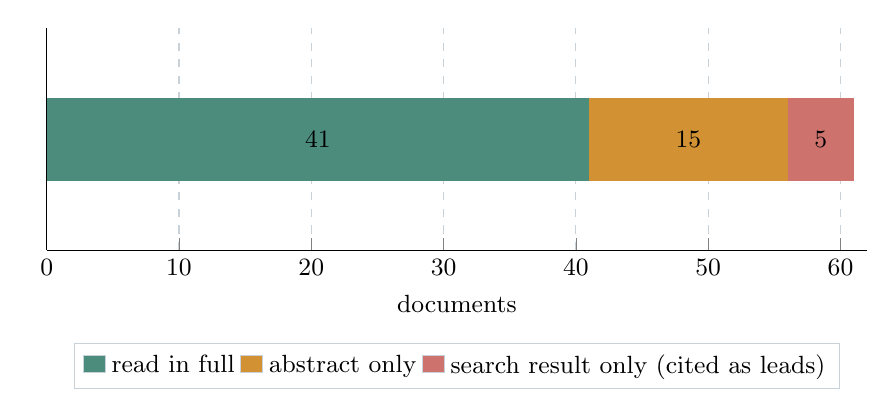
\begin{tikzpicture}
\begin{axis}[
  width=12cm, height=4.4cm,
  xbar stacked, bar width=30pt,
  xmin=0, xmax=62,
  xlabel={documents},
  xlabel style={font=\small},
  symbolic y coords={{sources}},
  ytick=data,
  yticklabels={},
  xticklabel style={font=\small},
  xmajorgrids, grid style={rule, dashed},
  legend style={font=\small, at={(0.5,-0.42)}, anchor=north, legend columns=3, draw=rule},
  axis lines*=left,
  nodes near coords, nodes near coords style={font=\small\bfseries, anchor=center},
]
\addplot[fill=standing!80, draw=none] coordinates {(41,{sources})};
\addplot[fill=partial!80, draw=none] coordinates {(15,{sources})};
\addplot[fill=killed!65, draw=none] coordinates {(5,{sources})};
\legend{read in full, abstract only, search result only (cited as leads)}
\end{axis}
\end{tikzpicture}
\end{center}

Every claim in this report about what a paper \emph{measured} rests on a document
read in full. Abstract-level sources are used only for claims about what a paper
\emph{is}. Search-result-only items appear in the bibliography as leads and are
labelled as such; none carries a verdict.

% ================================================================
\newpage
\section{Annotated bibliography}

Every entry carries a line describing how it differs. An entry without that line
would be a bookmark, not related work.

\subsection{Closest architectural prior art}

\begin{description}[leftmargin=0pt, style=unboxed, itemsep=6pt]

\item[1. Kurniawan, Ardian, Kiesling \& Ekelhart. \emph{AgCyRAG.}] RAGE-KG 2025 at
ISWC 2025, CEUR-WS Vol-4079, pp.~132--144. Workshop, non-archival. \readtag \\
\emph{Differs:} generates one of its two query languages with a language model while
predefining only the other; integrates at the prompt level with no cross-store join;
reports zero measurements over three demonstration questions.

\item[2. Kurniawan, Kiesling \& Ekelhart. \emph{CyKG-RAG.}] RAGE-KG 2024 at ISWC
2024, CEUR-WS Vol-3950. Workshop. \readtag \\
\emph{Differs:} the predecessor system --- three narrative walkthroughs, no question
set, no reference queries, no measurements; the authors state that comprehensive
evaluation is future work.

\item[3. Ozsoy. \emph{Toward Multi-Database Query Reasoning for Text2Cypher.}]
arXiv:2605.10373, 2026. Preprint; venue \unver. \readtag \\
\emph{Differs:} a roadmap that builds nothing, evidenced by seven hand-written
questions, whose multi-language example pairs a graph language with a
spreadsheet-style language.

\item[4. Wang, Jedema, Pandey, Krishnan, Lehmann \& Wu. \emph{UniQGen.}]
arXiv:2605.00845, 2026. Preprint. \readtag \\
\emph{Differs:} renders two query languages for the \textbf{same} store --- dual
rendering against one endpoint, not dispatch across two.

\item[5. Yun, Ye, Li, Li, Deng, Li \& Xiong. \emph{EICopilot.}] arXiv:2501.13746,
2025. Preprint. \abstag \\
\emph{Differs:} real natural-language-to-Gremlin, deployed, but one store, one
language, one domain, with no routing or federation.

\item[6. Dobriy, Bauer, Azzam, Banerjee \& Polleres. \emph{Agentic SPARQL.}]
arXiv:2603.06582, 2026. Preprint. \abstag \\
\emph{Differs:} genuine agent-driven federation, built on the standardisation of one
query language --- the cross-language problem is definitionally absent, and no merged
counterpart is constructed.

\item[7. \emph{Open Biomedical Knowledge Graphs at Scale (Samyama).}]
arXiv:2603.15080, 2026. Preprint; authors \unver. \abstag \\
\emph{Differs:} calls merging into one store ``federation''; one query language
throughout; its accuracy table compares interfaces rather than architectures.

\item[8. Sikos. \emph{Cybersecurity knowledge graphs.}] Knowledge and Information
Systems 65:3511--3531, 2023. Peer-reviewed survey. \readtag \\
\emph{Differs:} mentions federated queries once, uncited, illustrated by a
single-store query, with no open-problems section --- it does not establish the gap it
is cited for.

\item[9. Thakkar et al. \emph{Gremlinator.}] arXiv:1801.09556; ICSC 2020. Authors
\unver. \sniptag \\
\emph{Differs:} a query-language translator predating language models --- a component,
not a system, with no natural-language layer and no federation.

\item[10. Sivasubramaniam et al. \emph{SM3-Text-to-Query.}] arXiv:2411.05521, 2024.
Venue \unver. \abstag \\
\emph{Differs:} four query languages evaluated independently over four stores; no
query ever spans two stores.

\item[11. Vejvar \& Fujimoto. \emph{Spider4SSC.}] arXiv:2511.09354, 2025. \sniptag \\
\emph{Differs:} a matched-question dataset and a rule-based translator --- static
artifacts with no runtime and no live stores.

\item[12. Li \& Gupta. \emph{Natural Language to What?}] arXiv:2604.10776, 2026.
Preprint. \abstag \\
\emph{Differs:} names the terrain as open and builds nothing; useful for motivation,
harmless as prior art.
\end{description}

\subsection{Failure attribution and pipeline analysis}

\begin{description}[leftmargin=0pt, style=unboxed, itemsep=6pt]
\item[13. Leung, Belbahri, Sui, Labach, Zhang, Rose \& Cresswell.] EACL 2026,
pp.~3185--3207. Peer-reviewed. \readtag \\
\emph{Differs:} locates the earliest failing stage in a text pipeline with \textbf{no
planning stage}, and finds the answer-writing stage dominant --- the direct empirical
counterweight to the headline claim.

\item[14. \emph{Doctor-RAG.}] arXiv:2604.00865, 2026. Preprint; venue \unver. \readtag \\
\emph{Differs:} minimises over the earliest erroneous action for \textbf{repair},
reusing the valid prefix, and never asks whether the answer was still recoverable;
its distribution is image-only and \unver.

\item[15. Shah. \emph{Causal Agent Replay.}] arXiv:2606.08275, 2026. Preprint, single
author. \readtag \\
\emph{Differs:} owns the last-recoverable-step rule but validates on artificial test
cases and reports no finding about where losses concentrate in any real system.

\item[16. Ma et al.] arXiv:2509.08682, 2025. Preprint. \readtag \\
\emph{Differs:} reports attribution \emph{accuracy} against labels, never a
distribution of failures across stages, and has no recoverability criterion.

\item[17. Zhang, S. et al. \emph{Which Agent Causes Task Failures and When?}] ICML
2025 (Spotlight). Peer-reviewed. \sniptag\ (corroborated inside a retrieved paper) \\
\emph{Differs:} shows that machine-judged step attribution is unreliable (14.2\%
accuracy) --- an argument \textbf{for} mechanical location rather than a scoop of it.

\item[18. Zhang, G. et al. \emph{AgenTracer.}] arXiv:2509.03312, 2025. Preprint. \abstag \\
\emph{Differs:} substitutes ideal actions to build training data for a diagnosis
model, not stage-wise loss accounting in a knowledge-graph pipeline.

\item[19. Agrawal, Kumarage, Alghamdi \& Liu. \emph{Mindful-RAG.}] arXiv:2407.12216.
Preprint; venue \unver. \readtag \\
\emph{Differs:} the closest error taxonomy for this setting, but its categories are
assigned by human and machine judgement, with no mechanical location and no stage
percentages.

\item[20. Garani.] TrustNLP 2026 at ACL, pp.~413--424. Peer-reviewed workshop. \readtag \\
\emph{Differs:} a literature review with zero new measurements that grades the
evidence for planning failures as \emph{limited} --- a supporting citation, not a
threat.

\item[21. \emph{The Routing Plateau.}] arXiv:2606.07587, 2026. Preprint; authors
\unver. \readtag \\
\emph{Differs:} measures the gap between real and ideal routers (10--30 points), which
is selection quality, not a routing-versus-answering discrepancy.

\item[22. \emph{LogRouter.}] arXiv:2605.18015, 2026. Preprint; authors \unver. \readtag \\
\emph{Differs:} \textbf{contradicts} the routing sub-claim --- states the relationship
between routing accuracy and answer quality is direct.
\end{description}

\subsection{Templates against generic construction}

\begin{description}[leftmargin=0pt, style=unboxed, itemsep=6pt]
\item[23. Ding, Hu, Xu \& Qu.] EMNLP-IJCNLP 2019. Peer-reviewed. \readtag \\
\emph{Differs:} measures the coverage cost of templates and names the mechanism, but
never measures refusal and never leaves one database, so no reversal can appear.

\item[24. Gao, Lau \& Qi. \emph{SG-KBQA.}] EMNLP 2025, pp.~8753--8772. Peer-reviewed.
\abstag \\
\emph{Differs (from the summary only):} compares against other learned systems rather
than hand-written templates, on within-benchmark generalisation rather than
cross-structure transfer.

\item[25. Bast \& Haussmann (CIKM 2015); Zheng et al.\ (PVLDB 2018); Abujabal et al.\
(WWW 2017); Gu et al.\ (AKBC 2022); Scholak et al.\ (PICARD, EMNLP 2021).] All
peer-reviewed; records verified. \readtag \\
\emph{Differ:} establish that both templates-instead-of-parsing and constrained
generation are a decade old. PICARD in particular is the ``constrain rather than
eliminate'' objection that must be answered directly.

\item[26. Luo, Zhao, Haffari, Li, Gong \& Pan. \emph{Graph-constrained Reasoning.}]
ICML 2025, pp.~41540--41565. Peer-reviewed; results \unver. \readtag \\
\emph{Differs:} constrains generation to pre-encoded valid paths within one graph ---
the strongest form of the alternative approach, and the paper the architectural
argument must beat on its merits.
\end{description}

\subsection{Refusal and verification}

\begin{description}[leftmargin=0pt, style=unboxed, itemsep=6pt]
\item[27. Sawhney, Yadav, Bhattacharya \& Mausam.] Findings of ACL 2025.
Peer-reviewed. \readtag \\
\emph{Differs:} returns the query with ``no answer'' as a \emph{parse to be scored},
treats empty results as errors to repair, has no user and no provenance, and returns
nothing at all when the question cannot be expressed against the structure.

\item[28. Li, Appleby \& Suh. \emph{LinkQ.}] IEEE VIS 2024 short paper. Peer-reviewed.
\readtag \\
\emph{Differs:} never checks that the emitted query uses the supplied identifiers ---
that is delegated to the user --- and its evaluation is a five-person demonstration
with no benchmark.

\item[29. Deutch, Frost, Gilad et al.] The VLDB Journal 29(1), 2020. Peer-reviewed.
\abstag \\
\emph{Differs:} explains records that \textbf{are} in the result; refusal and empty
results are out of scope.

\item[30. Kang, Fu \& Zhao.] arXiv:2606.15833, 2026. Preprint; venue \unver. \abstag \\
\emph{Differs:} refuses when textual support for a fact is missing --- provenance-keyed
refusal, but the artifact is a retrieved passage, not an executed query returned to
the reader.

\item[31. Lee, Ludwig \& Glavic (PUG, PVLDB 2018); Bidoit et al.\ (NedExplain, EDBT
2014).] \sniptag \\
\emph{Differ:} the established literature on explaining why a record is \emph{missing}
from a query result --- with no natural-language layer and no refusal decision.
\textbf{The field to connect to; nobody has.}
\end{description}

\subsection{Evaluation methodology}

\begin{description}[leftmargin=0pt, style=unboxed, itemsep=6pt]
\item[32. Xu, Agrawal, Zouhar, Freitag \& Deutsch.] arXiv:2509.26600v2, 2026.
\textbf{Preprint only.} \readtag \\
\emph{Differs:} measures test-set-authorship bias for a \emph{machine} author,
attributed to stylistic similarity; never addresses a human team writing an
evaluation for its own system, and never controls for contamination.

\item[33. Singh, Fraser, Hooker et al. \emph{The Leaderboard Illusion.}] NeurIPS 2025.
Peer-reviewed. \sniptag \\
\emph{Differs:} selective submission and disclosure on a third-party leaderboard ---
reporting bias, with a neutral benchmark author.

\item[34. \emph{Measuring what Matters.}] NeurIPS 2025 Datasets \& Benchmarks.
Peer-reviewed. \sniptag \\
\emph{Differs:} diagnoses the problem class across 445 papers without isolating
developer authorship or attaching a number.

\item[35. \emph{Position: Benchmarking is Broken} (PeerBench).] arXiv:2510.07575.
Preprint. \abstag \\
\emph{Differs:} asserts the risk and measures nothing. \textbf{The paper that would
have scooped this and did not.}

\item[36. \emph{Benchmark Inflation: Retro-Holdouts.}] arXiv:2410.09247. Acceptance
\unver. \sniptag \\
\emph{Differs:} measures contamination --- the effect explicitly excluded --- but supplies
the methodological template for a same-system, different-author design.

\item[37. Koo et al.\ (CoBBLEr, Findings of ACL 2024); Wataoka et al.\
(arXiv:2410.21819).] \sniptag \\
\emph{Differ:} grader-side bias --- the grader favours its own text. The effect claimed
here is upstream, in who wrote the questions.

\item[38. \emph{Industry Sponsorship Bias}, Catalogue of Bias (Oxford); GRADE Notes 3,
J. Clin. Epidemiol.\ 2023.] \sniptag \\
\emph{Differ:} the mature, named, quantified version of the effect --- in clinical
trials. Nobody has ported it to machine-learning benchmarking. \textbf{Borrow the
frame.}
\end{description}

\subsection{Security benchmarks and question sets}

\begin{description}[leftmargin=0pt, style=unboxed, itemsep=6pt]
\item[39. Simoni, Fontanta, Saracino \& Mori. \emph{TITAN.}] arXiv:2510.14670, 2025.
Preprint; venue \unver. \readtag \\
\emph{Differs:} 88{,}209 pairs whose answers are chains of relationship names walked by
a general-purpose library --- no query language, no database, no execution scoring, no
CAPEC, no validation.

\item[40. Sharma et al.\ (SambaNova). \emph{AttackQA.}] OpenReview. Preprint. \readtag \\
\emph{Differs:} flat text retrieval, and its ``human question'' flag means a human
wrote the \textbf{generator script}. The canonical instance of the calibration trap.

\item[41. Cheng, Liu, Li, Song \& Gao. \emph{CTIConnect.}] KDD 2026. Peer-reviewed.
\readtag \\
\emph{Differs:} text-similarity retrieval with no query language and no reference
queries; questions are template-constrained machine syntheses that experts
\emph{verified} rather than wrote.

\item[42. Feng et al. \emph{CTIBench.}] NeurIPS 2024 Datasets \& Benchmarks (venue
\unver\ by fetch). \readtag \\
\emph{Differs:} 2{,}500 flat multiple-choice questions, machine-generated from source
pages with a sample corrected by hand; only 40 items manually collected; no graph, no
queries.

\item[43. Jing, Tang, Shi, Zheng, Nie, Wu, Yang \& Luo. \emph{SecBench.}]
arXiv:2412.20787, 2024. \textbf{Preprint --- no venue stated.} \readtag \\
\emph{Differs:} genuinely human-written contest questions, but organised into nine
self-devised domains with \textbf{no ATT\&CK, CAPEC or CWE grounding anywhere},
80.4\% Chinese, 90.8\% fact recall.

\item[44. Hamzić, Skopik, Landauer, Wurzenberger \& Rauber.] arXiv:2604.11419, 2026.
Preprint. \readtag \\
\emph{Differs:} narrative reports with no catalogue grounding; questions, reference
answers and grader are all machines; reference queries exist at generation time but
are never released or scored.

\item[45. Sanchez. MS thesis, Angelo State University, 2025.] Not peer-reviewed. \readtag \\
\emph{Differs:} 30 genuinely hand-written questions, but reference answers are prose
scored by text similarity, released only as a PDF appendix with visible
question-to-answer misalignments.

\item[46. Cazzaro, Lennon \& Quattoni. \emph{CyQuark.}] arXiv:2606.14325, 2026.
Preprint. \readtag \\
\emph{Differs:} zero security content; releases a generator rather than a benchmark;
its own 100-sample human audit finds only \textbf{65\% correct} --- the yardstick any
generation pipeline must beat.

\item[47. CypherBench; SpCQL; SynthCypher; MindTheQuery (EMNLP 2025); PIPE-Cypher;
KG2Cypher.] \sniptag \\
\emph{Differ:} real reference queries with execution scoring over general-knowledge,
film, sport, finance and enterprise databases --- \textbf{no security catalogue in any
of them}.
\end{description}

\subsection{Graph-query interface security}

\begin{description}[leftmargin=0pt, style=unboxed, itemsep=6pt]
\item[48. Szlobodnyik.] \emph{Analytics} (MDPI) 5(3):25, published 28 July 2026.
Peer-reviewed journal. \readtag \\
\emph{Differs:} it does not meaningfully differ --- it \textbf{is} Q8, minus a
security-catalogue schema, minus Gremlin, minus database-level permissions, and with
machine-written rather than analyst-written probes.

\item[49. CVE-2024-7042 --- query injection in a widely used open-source toolkit.] \sniptag \\
\emph{Differs:} a vulnerability record, not a research contribution --- cite as evidence
that the problem class occurs in practice.

\item[50. Vendor production guidance on read-only accounts, timeouts and result
limits.] \sniptag \\
\emph{Differs:} engineering folklore with no threat model and no measurement --- which
strengthens the case for a measurement paper.

\item[51. SafeClawBench; AgentSecBench; AgentSpec (ICSE 2026); IPIGuard; ToolEmu;
AgentDojo.] \sniptag \\
\emph{Differ:} generic agent tool-use and sandbox safety; none instruments a graph
query language, a structural boundary, or destructive-traversal semantics.
\end{description}

\subsection{Multi-source and multi-tenant retrieval}

\begin{description}[leftmargin=0pt, style=unboxed, itemsep=6pt]
\item[52. Arceo \& Narsing. \emph{Securing the Agent.}] ACM CAIS 2026. Peer-reviewed.
\readtag \\
\emph{Differs:} single shared index, three synthetic tenants, 300 fabricated
documents, and a failure test defined purely as ``was the user allowed to see this?''
--- an allowed record from the wrong source is never a violation.

\item[53. Mu \& Li.] arXiv:2605.28112, 2026. Preprint. \readtag \\
\emph{Differs:} the wrong source is wrong because it is \textbf{malicious}; framed as
an integrity rather than confidentiality failure, with no leakage measure.

\item[54. Burnat \& Davidson.] arXiv:2605.19847, 2026. Preprint. \readtag \\
\emph{Differs:} every query hits exactly one store by construction; cross-tenant
leakage is zero by design, and answer writing is explicitly out of scope.

\item[55. Wang, Khramtsova, Zhuang \& Zuccon. \emph{FeB4RAG.}] SIGIR 2024,
pp.~763--773 (metadata \unver\ by fetch). Peer-reviewed. \readtag \\
\emph{Differs:} measures source selection and result merging with standard ranking
scores; a full-text search for seven confidentiality-related terms returns
\textbf{zero matches}. The Q9 negative is now closed.

\item[56. PerKGQA; \emph{Privacy-protected RAG for KGQA} (arXiv:2508.08785); US Patent
11{,}062{,}700.] \sniptag \\
\emph{Differ:} per-user partitioning and anonymisation --- access control as an
architecture, never as a measured leakage rate, never in a multi-store fan-out.
\end{description}

% ================================================================
\newpage
\section{What is still open}

Five things this audit could not close. All are cheap to close and worth closing
before submission.

\begin{enumerate}[itemsep=6pt]
\item \textbf{Workshop proceedings were never enumerated directly.} The brief itself
      identifies workshop papers as where the scoop risk lives, and general web search
      indexes them poorly. \textbf{Manually sweep the 2026 workshop proceedings of the
      two main semantic-web conferences}, and watch the RAGE-KG workshop specifically
      --- the group with the closest architecture has twice said evaluation is future
      work.
\item \textbf{The primary template systems were not opened} --- QUINT, TeBaQA,
      QAnswer/WDAqua. TeBaQA claims portability across databases, and a buried
      precision-versus-coverage table there would narrow Q4 further.
\item \textbf{SG-KBQA (EMNLP 2025) is abstract-only.} Q4's adjudication cannot be
      final until its results section is read.
\item \textbf{arXiv's bulk search interface was unavailable throughout}, so no
      systematic field search was possible. This is the main structural gap in the Q1
      negative.
\item \textbf{Two circulating statistics remain untraced} and must not be used. See
      the Q3 section.
\end{enumerate}

\vspace{1.2cm}
\begin{center}
\rule{0.5\textwidth}{0.4pt}\\[4mm]
{\small Prepared 26 August 2026. Ninety-five distinct search queries across three
research vocabularies; forty-one documents retrieved and read in full; fifteen
retrieved at summary level; the remainder recorded as leads rather than findings.}
\end{center}

\end{document}
